\documentclass[11pt,a4paper]{article}
\usepackage[utf8]{inputenc}
\usepackage[T1]{fontenc}
\usepackage{amsmath,amssymb}
\usepackage{graphicx,booktabs,array,longtable}
\usepackage[margin=2.5cm]{geometry}
\usepackage{hyperref}
\usepackage{setspace}
\onehalfspacing
\setlength{\parskip}{0.4em}
\setlength{\parindent}{0pt}

\title{Late-Time Vacuum Decay as a Cosmological Reset: Coleman--De Luccia Tunneling, Reheating Constraints, and Consistency Boundaries}
\author{Leon Sandler \\ Independent Researcher, The Conscious Machine --- Independent Research, Northbrook, Illinois, USA \\ sandler.leon@gmail.com   ·   ORCID 0009-0007-4584-808X}
\date{}
\begin{document}
\maketitle

\begin{abstract}
A late-time transition of the present dark energy out of a metastable vacuum has been proposed as the seed of a new cosmological epoch. We test this proposal as a reset mechanism instead of assuming it. For a scalar potential with an explicit metastable minimum at the dark-energy scale, the O(4) Coleman--De Luccia bounce is computed in flat space and with gravity (shooting, an independent boundary-value solution, analytic de Sitter tails), with a numerical error budget, a check of the negative-mode structure and 18 executable consistency checks. All scales are set by the dark energy, so the gravitational parameter is $g = f^2/M_{\rm Pl}^2 \sim 10^{-60}$, gravitational corrections are $\sim10^{-59}$, the Hawking--Moss channel is irrelevant, and the decay is a flat-space process controlled by one number, the action $B = b(\eta)/\lambda$. The survival of the present vacuum is evaluated with the Lorentzian four-volume of our past light cone in the observed expansion history, $V_4 = 0.059\,H_\Lambda^{-4}$, which is 445 times smaller than the Euclidean four-sphere volume often used as a shortcut: the 95\% bound is $\Gamma/H_\Lambda^4 < 51$, so the survival condition is weak and the transition window is set by $B \simeq 287$, with the mean decay time running from $8.2\times10^{7}$ yr to beyond $10^{100}$ yr as $B$ increases by only $\sim212$. For the stated priors, which define a parameter space and not probabilities for our universe, 14.8\% of the prior volume lies above the survival bound, 0.8\% decays within $10^{20}$ yr, and 80.4\% shows no decay within $10^{100}$ yr. Within explicit assumptions (one scalar field, minimal coupling, no inflationary stage) the nucleated region reheats to at most $2.2$ meV, $4.6\times10^{8}$ times below nucleosynthesis; this is not an energy-conservation statement alone: the open interior stays curvature dominated and a hot big bang at $t \sim 1$ s would require a parent energy scale at least 41 orders of magnitude above the Planck scale. A matter trigger requires a fractional change of the matter mass between the two vacua of $\Delta\ln m \gtrsim 8.9\times10^{-4}$, that is a linear coupling $\beta \sim 10^{26}$--$10^{29}$ or a quadratic coupling scale of tens of meV; screened couplings are not excluded by this paper. A cyclic reset by decay of the present dark energy is therefore not supported in this framework; consistency conditions and observational tests are listed separately.
\end{abstract}
\noindent\textbf{Keywords:} \emph{false vacuum decay; Coleman--De Luccia instanton; de Sitter space; dark energy; reheating; cyclic cosmology; past light cone; falsifiability}

\section{Introduction}
In the standard cosmological model the late universe approaches de Sitter space: matter and radiation dilute, and a positive vacuum energy $\rho_\Lambda$ remains. If that energy is not an exact cosmological constant but the energy of a metastable scalar vacuum, the vacuum can decay by quantum tunneling through a Coleman--De Luccia (CDL) instanton [1]. It has been suggested that such a late-time transition could reset the cosmological history, so that the long-term evolution is cyclic rather than terminal; cyclic and bouncing proposals are discussed in [2, 3, 4, 5]. Two things must be kept apart. The formation of a bubble universe is not a cyclic cosmology: a cycle needs a mechanism that connects successive epochs. The question tested here is narrower and can be answered by calculation: can the tunneling of the present dark energy produce a new hot, expanding epoch? That requires a specified metastable minimum, the tunneling action including gravity, a rate compared with the observed expansion history, and the interior of the nucleated region followed to see whether it can become a hot big bang.

Three claims are tested. (i) A scalar potential with a metastable minimum at the dark-energy scale can nucleate bubbles of lower-energy vacuum at a rate that is neither negligible nor already excluded. (ii) The nucleated region reheats into a hot expanding universe. (iii) The transition is triggered, or enhanced, by the dilution of matter in the late universe. The analysis is conditional: it takes the dark-energy density as the false-vacuum energy and asks what follows. The result is a quantitative consistency and exclusion analysis, not a new cosmological mechanism.

The contributions are the following.

\begin{itemize}\item A reproducible map from the parameters of an explicit scalar potential to cosmological decay times, with a numerical error budget, an independent boundary-value solution, the negative-mode structure of the bounce, the thin-wall, Parke and Hawking--Moss limits, and a treatment of the prefactor as a systematic uncertainty (Sections 2--4).
\item A joint analysis of nucleation, survival and the post-transition energy budget, with the survival of the present vacuum evaluated on the Lorentzian past light cone of the observed expansion history (Section 4.2), and a statement of which energy sources the reheating bound excludes by geometry and which only by energy conservation (Section 5).
\item Explicit conditions that separate a late-time vacuum transition from a viable cosmological restart, divided into internal consistency conditions and observational tests (Section 7), and a model-independent requirement on any matter coupling that could trigger the transition (Section 6).
\end{itemize}
\subsection{Relation to previous work}
The ingredients are established, and the paper claims novelty only for the specific combination and the quantitative results for the dark-energy vacuum. Table 1 states for each ingredient what is known, what is used from the literature and what is computed here.

\begin{table}[htbp]\centering\small
\caption{Closest literature and what this paper adds.}
\begin{tabular}{>{\raggedright\arraybackslash}p{0.255\dimexpr\textwidth-6\tabcolsep\relax}>{\raggedright\arraybackslash}p{0.373\dimexpr\textwidth-6\tabcolsep\relax}>{\raggedright\arraybackslash}p{0.373\dimexpr\textwidth-6\tabcolsep\relax}}
\toprule
Ingredient & Established (references) & This paper \\ \midrule
Bounce, thin wall, gravity, Hawking--Moss & Coleman; Callan--Coleman; CDL; Hawking--Moss; Parke; Jensen--Steinhardt; Hackworth--Weinberg [6, 7, 1, 8, 9, 10, 11] & Used as validation limits. New: an explicit dark-energy-scale potential, $g\sim10^{-60}$, and a numerical error budget and negative-mode check (Section 3). \\
Prefactor of the rate & Determinant methods [12, 13] & Not recomputed; treated as a systematic uncertainty with a stated spread and shown to enter $B_c$ additively (Section 4.3). \\
Survival from the past light cone & Standard for the electroweak vacuum [14, 15]; percolation [16, 17] & Applied to the dark-energy vacuum with the observed expansion history: $V_4=0.059\,H_\Lambda^{-4}$, 445 times below the Euclidean four-sphere (Section 4.2). \\
Open interior and reheating & Open universes from bubbles need an inflationary stage [18, 19, 20] & Quantified for the dark-energy scale: curvature parameter, e-folds and the parent scale needed for a hot epoch (Section 5.3). \\
Cyclic and bouncing models & [2, 3, 4, 5] & These supply the reset by other means; here one proposed mechanism, tunneling of the present dark energy, is tested. \\
Landscape and bubble collisions & [21, 22, 20, 23, 24] & Observable signals need $\Gamma/H^4=O(1)$; the width of that window in $B$ and its prior mass are computed (Section 4.5). \\
Matter couplings and screening & [25, 26] & A coupling-independent requirement, $\Delta\ln m$, and its translation to linear and quadratic couplings (Section 6). \\
\bottomrule
\end{tabular}
\end{table}
\section{Scalar effective theory and the potential}
We consider a real scalar field minimally coupled to Einstein gravity,

\begin{equation}
S=\int d^4x\sqrt{-g}\left[\frac{M_{\rm Pl}^2}{2}R-\frac12 g^{\mu\nu}\partial_\mu\varphi\,\partial_\nu\varphi-V(\varphi)\right]
\end{equation}
where $M_{\rm Pl}$ is the reduced Planck mass. The false vacuum has the energy density $V_f = V(\varphi_f)$, which is identified with the observed dark energy, $V_f = \rho_\Lambda = 2.55\times10^{-47}$ $\mathrm{GeV}^4$ (quarter-root 2.25 meV; Planck 2018 [27], $H_0 = 67.66\ \mathrm{km\,s^{-1}\,Mpc^{-1}}$, $\Omega_\Lambda = 0.6889$). The asymptotic de Sitter rate is $H_\Lambda = \sqrt{V_f/3}/M_{\rm Pl} = 1.20\times10^{-42}$ GeV, so that $H_\Lambda^{-1} = 17.4$ Gyr, and $M_{\rm Pl}^4/V_f = 1.38\times10^{120}$, with $\ln(M_{\rm Pl}^4/V_f) = 276.6$. A microscopic origin of the potential is not assumed.

A single dimensionless family covers the generic metastable case. With $x = \varphi/f$,

\begin{equation}
V(\varphi)=V_t+f^4\lambda\left[\frac{(x^2-1)^2}{8}+\frac{\eta\,x}{2}-p_{\min}(\eta)\right],\qquad x^3-x+\eta=0\ \Rightarrow\ x_t<x_{\rm top}<x_f
\end{equation}
where $p_{\min}$ is the value of the bracket at the true minimum, so that $V(\varphi_t) = V_t$. The tilt $\eta$ lifts the degeneracy of the two wells; a false minimum exists only for $\eta < \eta_c = 2/(3\sqrt3) = 0.3849$. The energy difference and the barrier height above the false minimum are

\begin{equation}
\Delta V=V_f-V_t=f^4\lambda\,\delta(\eta),\qquad V_{\rm top}-V_f=f^4\lambda\,\beta(\eta),\qquad \delta\simeq\eta\ (\eta\ll1)
\end{equation}
The motivation for this family is minimality. A quartic with a small linear term is the simplest renormalizable potential with a metastable minimum and was the standard example in the original treatments of vacuum decay [6, 1]; it has three parameters with direct meaning, the quartic coupling $\lambda$, the tilt-to-barrier ratio $\eta$ and the scale $f$, and the latter is fixed by the dark energy. The coupling is restricted to $10^{-2}\le\lambda\le4\pi$, the upper limit being the perturbative-unitarity bound for a quartic interaction and the lower limit an arbitrary but wide cut that is varied in Section 4.5; the tilt is restricted to $0.03\le\eta\le0.38$, which excludes the nearly degenerate case, where $B\propto\eta^{-3}$ is so large that the transition is irrelevant, and ends just below the point where the minimum disappears. Other potentials change $b(\eta)$ and the interior energy fraction but not the scales that decide the results (Section 8). A scalar with a mass of the order of meV is technically unnatural without a protecting symmetry; this is a known property of every quintessence-like model and is not addressed here.

The choice $V_t = 0$ (decay to a Minkowski vacuum, $r_L \equiv V_f/\Delta V = 1$) is the baseline, because it maximizes the energy released to the interior for a given $V_f$ when $V_t\ge0$; $V_t < 0$ (anti-de Sitter) and $V_t > 0$ are considered in Sections 5.3 and 4.5. The scale $f$ is not free: it is fixed by $V_f = \rho_\Lambda$, $f^4 = \rho_\Lambda/(r_L\lambda\delta)$. For $\lambda = 1$ and $\eta = 0.3$ one finds $f = 3.05$ meV and a field excursion of $5.8$ meV, that is, the dark-energy scale. The gravitational parameter is then fixed too,

\begin{equation}
g\equiv\frac{f^2}{M_{\rm Pl}^2}=\sqrt{\frac{V_f/M_{\rm Pl}^4}{r_L\,\lambda\,\delta(\eta)}}
\end{equation}
which takes the values $6.4\times10^{-61}$ to $2.7\times10^{-60}$ over the benchmark parameters of Table 4. Gravity is therefore a $10^{-60}$ effect in every equation below that does not contain the large number $M_{\rm Pl}^4/V_f$.

\section{The Euclidean bounce, with and without gravity}
\subsection{Equations and action}
The O(4)-symmetric Euclidean metric $ds^2 = d\xi^2 + \rho(\xi)^2 d\Omega_3^2$ gives the CDL equations [1]

\begin{equation}
\varphi''+3\frac{\rho'}{\rho}\varphi'=\frac{dV}{d\varphi},\qquad \rho'^2=1+\frac{\rho^2}{3M_{\rm Pl}^2}\left(\frac12\varphi'^2-V\right)
\end{equation}
with $\varphi'(0)=0$ and regularity at the second pole of the compact de Sitter geometry. On shell, the action of the bounce relative to the false vacuum is

\begin{equation}
B=S_E[{\rm bounce}]-S_E[{\rm false}],\quad S_E=4\pi^2\int d\xi\,\left(\rho^3V-3M_{\rm Pl}^2\rho\right),\quad S_E^{\rm dS}=-\frac{24\pi^2M_{\rm Pl}^4}{V_f}
\end{equation}
In the flat-space limit $B=2\pi^2\int dr\,r^3\,[\tfrac12\varphi'^2+V-V_f]$, and for a thin wall $B = 27\pi^2\sigma^4/(2\Delta V^3)$ with $R_c = 3\sigma/\Delta V$, $\sigma = \int\sqrt{2V}\,d\varphi$ [6]. With the field in units of $f$ and lengths in units of $(\sqrt\lambda f)^{-1}$ the flat-space action is $B = b(\eta)/\lambda$ exactly, and gravity enters only through $g$.

The Hawking--Moss action is $B_{\rm HM} = 24\pi^2 M_{\rm Pl}^4(1/V_f - 1/V_{\rm top})$ [8]; an oscillating CDL bounce requires $|V''_{\rm top}| > 4H^2$ [10, 11], which fails for sufficiently flat potentials or strong gravity.

\subsection{Numerical method and validation}
The bounce is found by shooting on the central field value with overshoot/undershoot classification (adaptive eighth-order Runge--Kutta, relative tolerance $10^{-11}$) [28, 29, 30], with the equations integrated through the wall and the action accumulated along the solution. For the gravitational problem the tail of the bounce outside the wall follows the false-vacuum de Sitter geometry $\rho = \sin(H\xi)/H$ toward the second pole, and the difference from the background action is taken analytically there, which avoids the cancellation of terms of order $1/g^2$. In the thin-wall regime shooting is exponentially sensitive to the initial condition, so an independent collocation boundary-value solver is used for $\eta < 0.1$, and the two agree to $2\times10^{-9}$ where both apply. The analytic thin-wall formula with gravity [9] serves as a further check of the gravitational suppression. Table 2 lists the checks of the bounce; the complete suite has 18 checks, all executed by a script distributed with the paper.

\begin{table}[htbp]\centering\small
\caption{Executable consistency checks of the numerical bounce.}
\begin{tabular}{>{\raggedright\arraybackslash}p{0.500\dimexpr\textwidth-4\tabcolsep\relax}>{\raggedright\arraybackslash}p{0.500\dimexpr\textwidth-4\tabcolsep\relax}}
\toprule
Check & Result \\ \midrule
Thin-wall limit: $B/B_{\rm thin}$ as $\eta\to0$ & 0.9943 at $\eta=0.03$, 0.9773 at 0.06 (monotone) \\
Shooting versus boundary-value solver & max relative difference $1.8\times10^{-9}$ (7 cases) \\
Scaling $B=b(\eta)/\lambda$ & max relative difference $9.8\times10^{-13}$ \\
de Sitter action $-24\pi^2M^4/V_f$ & relative difference $4\times10^{-16}$ \\
Friedmann constraint along the bounce & max residual $5.3\times10^{-12}$ \\
Gravitational suppression against the analytic thin-wall (Parke) value & agree to 1.5\% in $B/B_{\rm flat}$ (4 points) \\
Hawking--Moss consistency & 84 bounces found in 98 grid points; none with $|V''|<4H^2$; none above $B_{\rm HM}$ \\
Interpolation of $b(\eta)$ off the table & max relative error $6.6\times10^{-5}$ \\
Derrick identity $2T+4U=0$ for the bounce & residual $1.4\times10^{-7}$ at the worst of four tilts \\
\bottomrule
\end{tabular}
\end{table}
\begin{figure}[htbp]\centering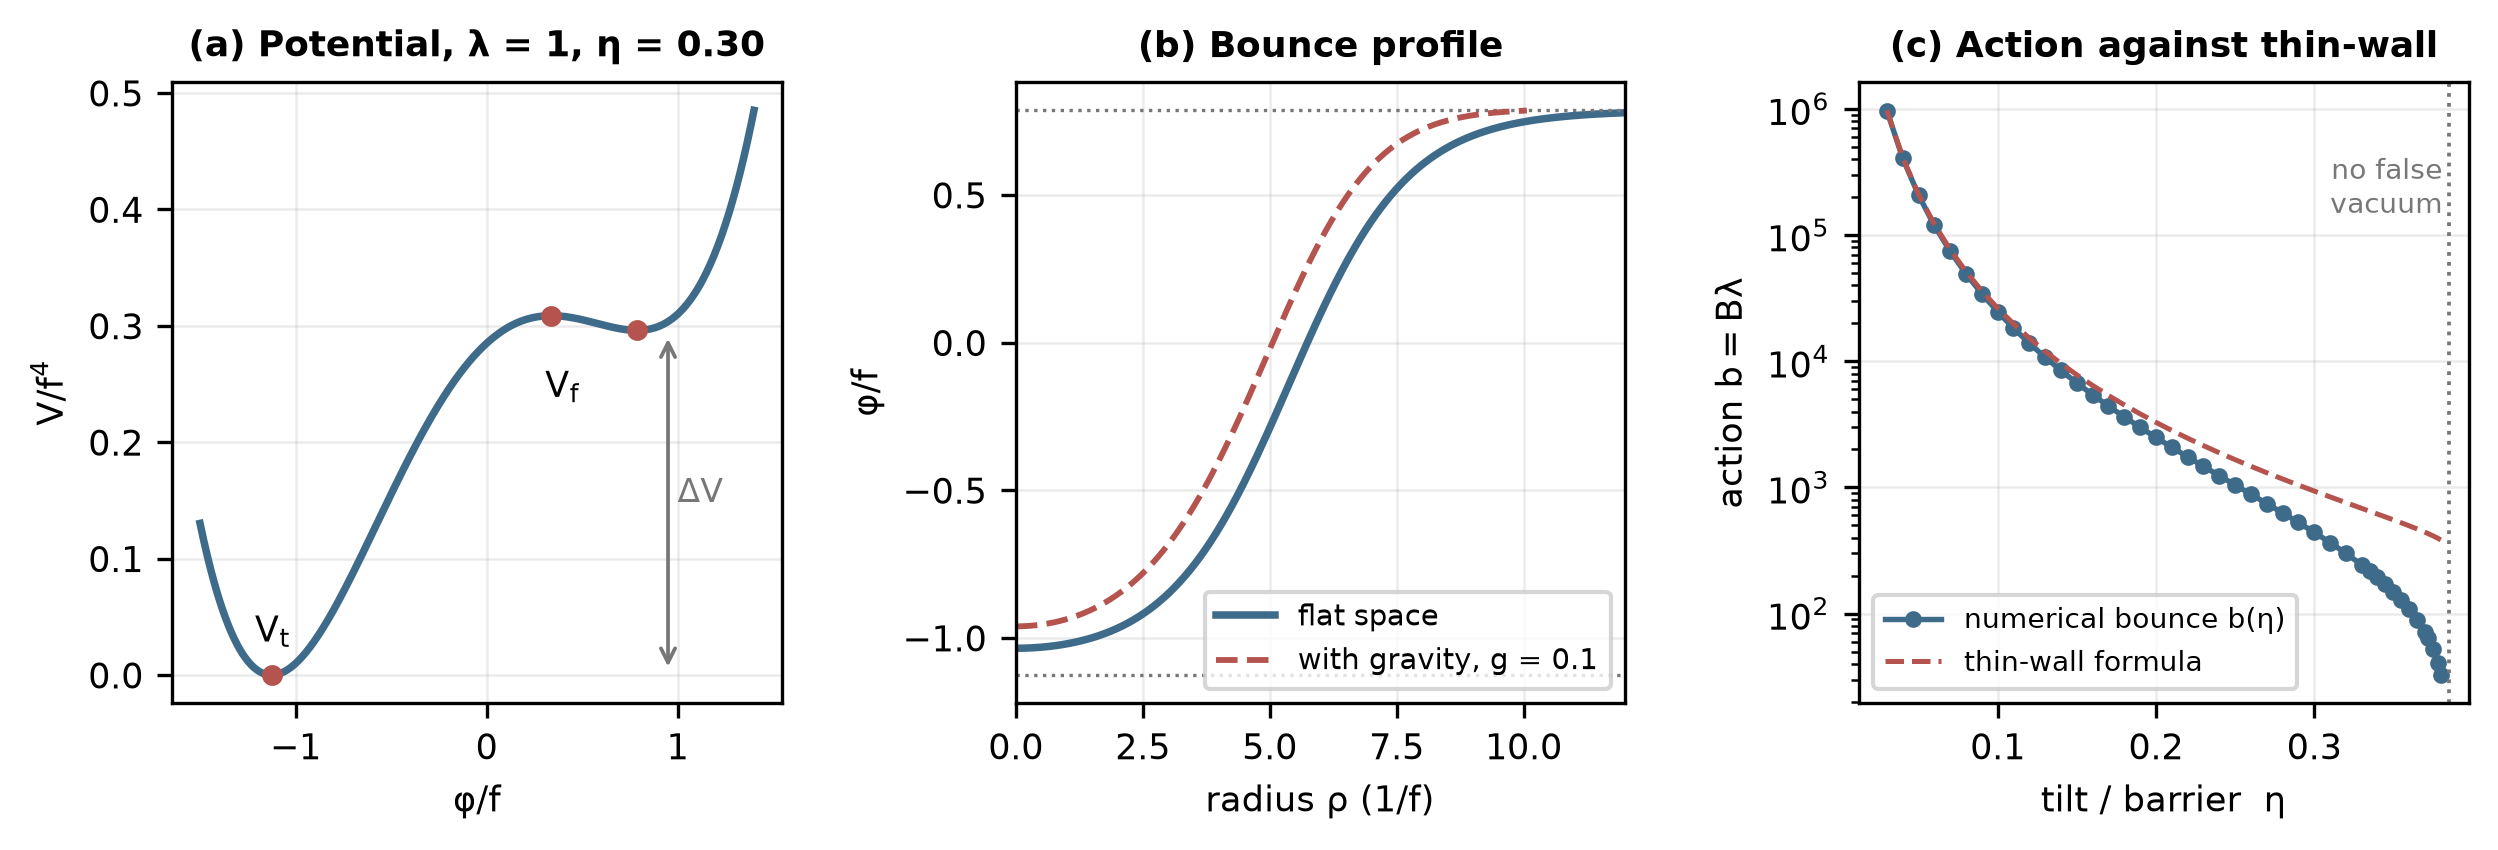
\includegraphics[width=1.00\textwidth]{../figures/fig1_potential_bounce.png}\caption{(a) The potential for $\lambda=1$, $\eta=0.30$. (b) The bounce profile in flat space and with gravity ($g=0.1$). (c) The numerical action $b(\eta)=B\lambda$ against the thin-wall formula; the false minimum disappears at $\eta_c=0.385$.}\end{figure}
\subsection{Error budget and negative modes}
Table 3 lists how the flat-space action changes when each numerical choice is varied: the integrator tolerance and the integrator itself, the quadrature of the action integral, the tolerance of the bisection on the central field value, the truncation of the domain, and, for the boundary-value solution, the tolerance, the initial mesh and the padding of the domain. At the production settings the numerical uncertainty of $B$ is below $1\times10^{-8}$, many orders below the uncertainty of the prefactor ($\delta\ln\Gamma=O(1)$) and below the precision of any quantity compared with the data. The only sensitive setting is the bisection: a tolerance of $10^{-6}$ in the central field value changes $B$ by up to $1\times10^{-4}$ in the thin-wall regime, which is why $10^{-13}$ is used.

\begin{table}[htbp]\centering\small
\caption{Numerical error budget of the flat-space action (largest relative change of $B$ over the tilts studied).}
\begin{tabular}{>{\raggedright\arraybackslash}p{0.346\dimexpr\textwidth-6\tabcolsep\relax}>{\raggedright\arraybackslash}p{0.316\dimexpr\textwidth-6\tabcolsep\relax}>{\raggedright\arraybackslash}p{0.338\dimexpr\textwidth-6\tabcolsep\relax}}
\toprule
Source & Range explored & Largest change \\ \midrule
Integrator tolerance (DOP853) & $10^{-8}$ to $10^{-13}$ (production $10^{-11}$) & $3\times10^{-9}$ ($2\times10^{-11}$ for tolerance $\le10^{-10}$) \\
Integrator & DOP853, RK45, LSODA, Radau & $3\times10^{-10}$ \\
Quadrature of the action & $2\times10^4$ to $2\times10^6$ points & $2\times10^{-14}$ \\
Bisection on the central value & $10^{-6}$ to $10^{-13}$ (production $10^{-13}$) & $1\times10^{-4}$ ($1\times10^{-8}$ for tolerance $\le10^{-10}$) \\
Truncation of the domain & action cut at $r_{1/2}+k/m_f$, $k$ up to 16 & $1\times10^{-6}$ at the largest radius reached \\
Boundary-value solver: tolerance, mesh, padding & $10^{-6}$ to $10^{-10}$; 500 to 8000 nodes; 10 to 120 & $3\times10^{-12}$ \\
Shooting against boundary-value solution & $\eta=0.10$ & $2\times10^{-9}$ \\
Gravity coefficient $\kappa(g\to0)$ & integrators, tolerances, quadrature & $\kappa=3.6407$, spread $3\times10^{-5}$ \\
\bottomrule
\end{tabular}
\end{table}
A CDL bounce is a saddle point with exactly one negative mode, which is what allows $\mathrm{Im}\,E$ to be interpreted as a decay rate [6, 7]. For $\eta=0.05$, 0.15, 0.30 and 0.36 the spectrum of $-\nabla_4^2+V''(\varphi_b)$ was computed in the angular sectors $l=0,\dots,4$ (with $\psi=r^{-3/2}u$ the radial operator is $-u''+[(l(l+2)+3/4)/r^2+V'']u$, discretized on 30000 points). In every case the $l=0$ sector has exactly one negative eigenvalue (lowest values $-0.002$, $-0.024$, $-0.21$, $-0.74$ in units of the false-vacuum mass squared), the $l=1$ sector has the lowest eigenvalue consistent with the four translational zero modes (at most $2\times10^{-7}$ of $m_f^2$ in magnitude) and none is negative, no eigenvalue is negative for $l\ge2$, the field is monotonic, so that $\varphi-\varphi_f$ has no node, and the Derrick identity holds to $1\times10^{-7}$. With gravity the negative-mode problem is subtle and has been discussed in the literature [31]; here $g\sim10^{-60}$, the operator differs from its flat-space form by a relative $O(g)$, and the flat-space structure applies. The gravitational spectrum was not computed for large $g$.

Corrections of relative size $10^{-59}$ cannot be resolved in double precision, and the paper does not claim to resolve them. The flat-space action is computed with no gravity at all; the gravitational correction is the linear response $B=B_{\rm flat}(1-\kappa g)$ with $\kappa(g\to0)=3.641$, obtained from $g=10^{-3}$ and $2\times10^{-3}$ with the linear extrapolation $\kappa_0=2\kappa(10^{-3})-\kappa(2\times10^{-3})$ (the two values differ by 2.6\%, the curvature of $B(g)$) and stable to $3\times10^{-5}$ across integrators. At $g\sim10^{-60}$ the correction $\kappa g\sim9.7\times10^{-60}$ is some 59 orders of magnitude below every other uncertainty of the rate, so what matters is only that gravity enters as a small smooth perturbation, which the Hawking--Moss criterion confirms independently (Section 3.4).

\subsection{Gravitational corrections and the Hawking--Moss limit}
Fig. 2a shows the ratio $B(g)/B_{\rm flat}$ computed on a grid of $g$ and $\eta$. For small $g$ the suppression is linear, $B = B_{\rm flat}(1-\kappa g)$ with $\kappa = 3.5$ to $6.7$ for $0.12 \le \eta \le 0.37$ (measured at $g = 10^{-3}$; below that the cancellation of the $1/g^2$ terms limits the numerical precision to about $10^{-4}$ in $B/B_{\rm flat}$). The suppression grows with $g$ as the bubble approaches the Hubble radius, and for $g \gtrsim 1$ no oscillating bounce is found: the numerical existence agrees with the condition $|V''_{\rm top}|/4H^2>1$ (Fig. 2b), which is satisfied everywhere a bounce was found.

\begin{figure}[htbp]\centering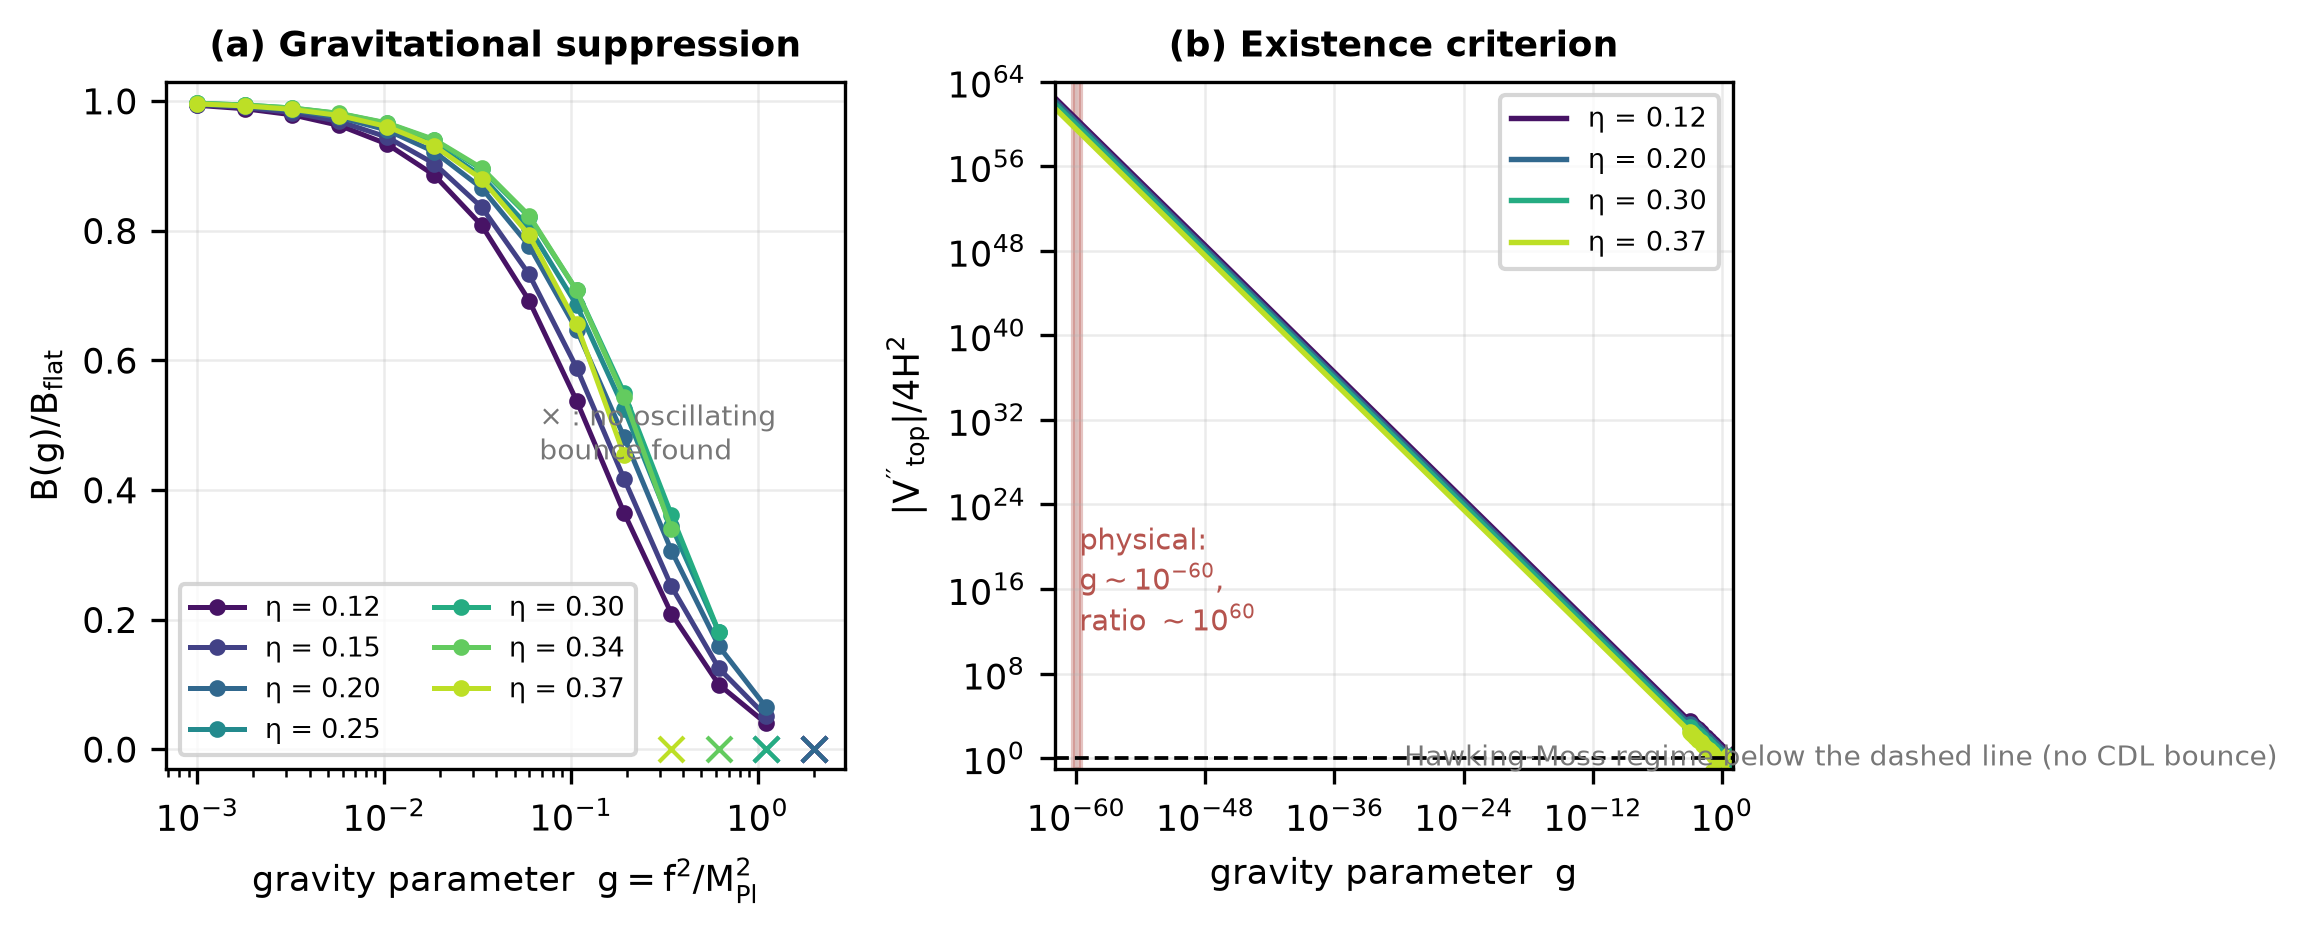
\includegraphics[width=1.00\textwidth]{../figures/fig2_gravity_hawking_moss.png}\caption{(a) Gravitational suppression of the action for several tilts; crosses mark the grid points at which no oscillating bounce was found. (b) The Hawking--Moss criterion $|V''_{\rm top}|/4H^2$ against $g$ (lines, analytic; markers, numerical bounce found/not found). The shaded band is the physical value fixed by the dark energy, $g\sim10^{-60}$.}\end{figure}
At the physical $g\sim10^{-60}$ the relative gravitational correction is $\kappa g\sim9.7\times10^{-60}$, the Hawking--Moss criterion is satisfied by a factor $\sim10^{59}$--$10^{60}$, the Hawking--Moss action is $\ln B_{\rm HM}\simeq279$ (an exponent of $10^{121}$), and the bubble radius is $\sim2\times10^{-30}$ of the Hubble radius. Gravity and the Hawking--Moss channel play no role in a decay of the present dark energy within this class of potentials. They matter only if $f\gtrsim 0.3 M_{\rm Pl}$, which with $V_f$ fixed requires $V_f/f^4\lesssim9\times10^{-119}$, a barrier $\gtrsim1\times10^{118}$ times the vacuum energy, and an action beyond any consequence for the transition.

\section{Nucleation rate and survival in the observed universe}
\subsection{The rate}
The rate per unit four-volume is $\Gamma/V_4 = A\,e^{-B}$ [6, 7]. In the rescaled variables $\Gamma/V_4 = K f^4\lambda^2 e^{-B}$, where $K = (B/2\pi)^2 D$ contains the four translational zero modes and an unknown dimensionless factor $D$ from the remaining fluctuation determinant. Dividing by $H^4 = V_f^2/(9M_{\rm Pl}^4)$ and using $f^4 = V_f/(r_L\lambda\delta)$,

\begin{equation}
\frac{\Gamma}{H^4}=\frac{9K\lambda}{r_L\,\delta(\eta)}\,\frac{M_{\rm Pl}^4}{V_f}\,e^{-B(\lambda,\eta)}
\end{equation}
The large number $M_{\rm Pl}^4/V_f = 1.38\times10^{120}$ is the number of Planck-volume cells in a Hubble four-volume. It compensates an action of $B \simeq \ln(M_{\rm Pl}^4/V_f) = 276.6$ plus the logarithm of the prefactor. Setting $\Gamma/H^4 = 1$ gives the critical action

\begin{equation}
B_c=\ln\frac{M_{\rm Pl}^4}{V_f}+\ln\frac{9K\lambda}{r_L\,\delta},\qquad B_c\simeq 287\ \ (\text{median over the prior; 5--95\% range }280\text{--}294)
\end{equation}
For a mean time to nucleation, an observer in the asymptotic de Sitter space sees the past-cone four-volume grow at the rate $(4\pi/3)H^{-3}$, so the mean time for one Hubble patch to nucleate a bubble is $t_{\rm dec} = H^{-1}/[(4\pi/3)\Gamma/H^4]$ for $\Gamma/H^4\ll1$. For $\lambda=1$, $\eta=0.30$ the action is $B=441$ and the mean decay time is $10^{76}$ yr; at $\eta=0.32$ ($B=301$) it is $10^{15}$ yr; at $\eta=0.34$ ($B=194$) the rate is so large that the vacuum would not have survived and the model is excluded (Table 4).

\begin{table}[htbp]\centering\small
\caption{Benchmark potentials with the dark-energy density as false-vacuum energy ($r_L=1$). $f$ is the field scale, $g=f^2/M_{\rm Pl}^2$, $\delta_B$ the relative gravitational correction to $B$, and $R_b/R_H$ the bubble radius over the Hubble radius.}
\begin{tabular}{llllllllll}
\toprule
$\lambda$ & $\eta$ & $f$ (meV) & $B$ & $\ln\Gamma/H^4$ & $\log_{10}t_{\rm dec}$ (yr) & $g$ & $\delta_B$ & $|V''_{\rm top}|/4H^2$ & $R_b/R_H$ \\ \midrule
1 & 0.30 & 3.05 & 441 & -153 & 76 & $1.6\times10^{-60}$ & $5.6\times10^{-60}$ & $5.3\times10^{59}$ & $2.6\times10^{-30}$ \\
1 & 0.32 & 3.00 & 301 & -13 & 15 & $1.5\times10^{-60}$ & $5.4\times10^{-60}$ & $4.6\times10^{59}$ & $2.5\times10^{-30}$ \\
1 & 0.34 & 2.96 & 194 & 93 & -31 & $1.5\times10^{-60}$ & $5.3\times10^{-60}$ & $3.8\times10^{59}$ & $2.3\times10^{-30}$ \\
0.3 & 0.34 & 4.00 & 645 & -357 & 165 & $2.7\times10^{-60}$ & $9.7\times10^{-60}$ & $2.1\times10^{59}$ & $3.2\times10^{-30}$ \\
3 & 0.25 & 2.42 & 349 & -60 & 36 & $9.9\times10^{-61}$ & $3.8\times10^{-60}$ & $1.2\times10^{60}$ & $2.3\times10^{-30}$ \\
10 & 0.18 & 1.94 & 363 & -72 & 41 & $6.4\times10^{-61}$ & $3.2\times10^{-60}$ & $2.9\times10^{60}$ & $2.2\times10^{-30}$ \\
\bottomrule
\end{tabular}
\end{table}
\subsection{Survival of the present vacuum: the past light cone}
A bubble nucleated at an event $p$ expands at essentially the speed of light and reaches an observer at $O$ if and only if $p$ lies in the causal past of $O$. If nucleations are Poisson distributed with rate $\Gamma$ per unit four-volume, the probability that none has occurred in the past light cone of the present observer is [14, 15]

\begin{equation}
P_{\rm surv}=e^{-\Gamma V_4},\qquad V_4=\frac{4\pi}{3}\int_0^{t_0}dt\,a(t)^3\chi(t)^3,\qquad \chi(t)=\int_t^{t_0}\frac{dt'}{a(t')}
\end{equation}
with $\chi$ the comoving distance of the light cone at time $t$ in a flat universe. A common order-of-magnitude shortcut uses the Euclidean volume of the de Sitter four-sphere, $8\pi^2/(3H^4)$; that is not the four-volume of any region of the observed spacetime, and it overstates $V_4$ by the factor given below. The observed history is $H^2=H_0^2(\Omega_ma^{-3}+\Omega_ra^{-4}+\Omega_\Lambda)$ with $\Omega_\Lambda=0.6889$, $\Omega_r=9.14\times10^{-5}$ (from $T_{\rm CMB}$ and $N_{\rm eff}=3.046$) and $\Omega_m=0.3110$. Two independent quadratures give $V_4=0.12457\,H_0^{-4}=0.0591\,H_\Lambda^{-4}$, agreeing to $1\times10^{-13}$; the result is converged in the lower cutoff of the scale factor and in the grid to $10^{-11}$ and reproduces the analytic Einstein--de Sitter value to $2\times10^{-13}$ (check V14). The Euclidean volume is $26.3\,H_\Lambda^{-4}$, 445 times larger. Of $V_4$, 35\% comes from events at redshift below 1, 73\% below 2 and 97\% below 5 (Fig. 3); the uncertainty from $\Omega_\Lambda$ at the Planck $1\sigma$ level is about 3.5\%.

\begin{figure}[htbp]\centering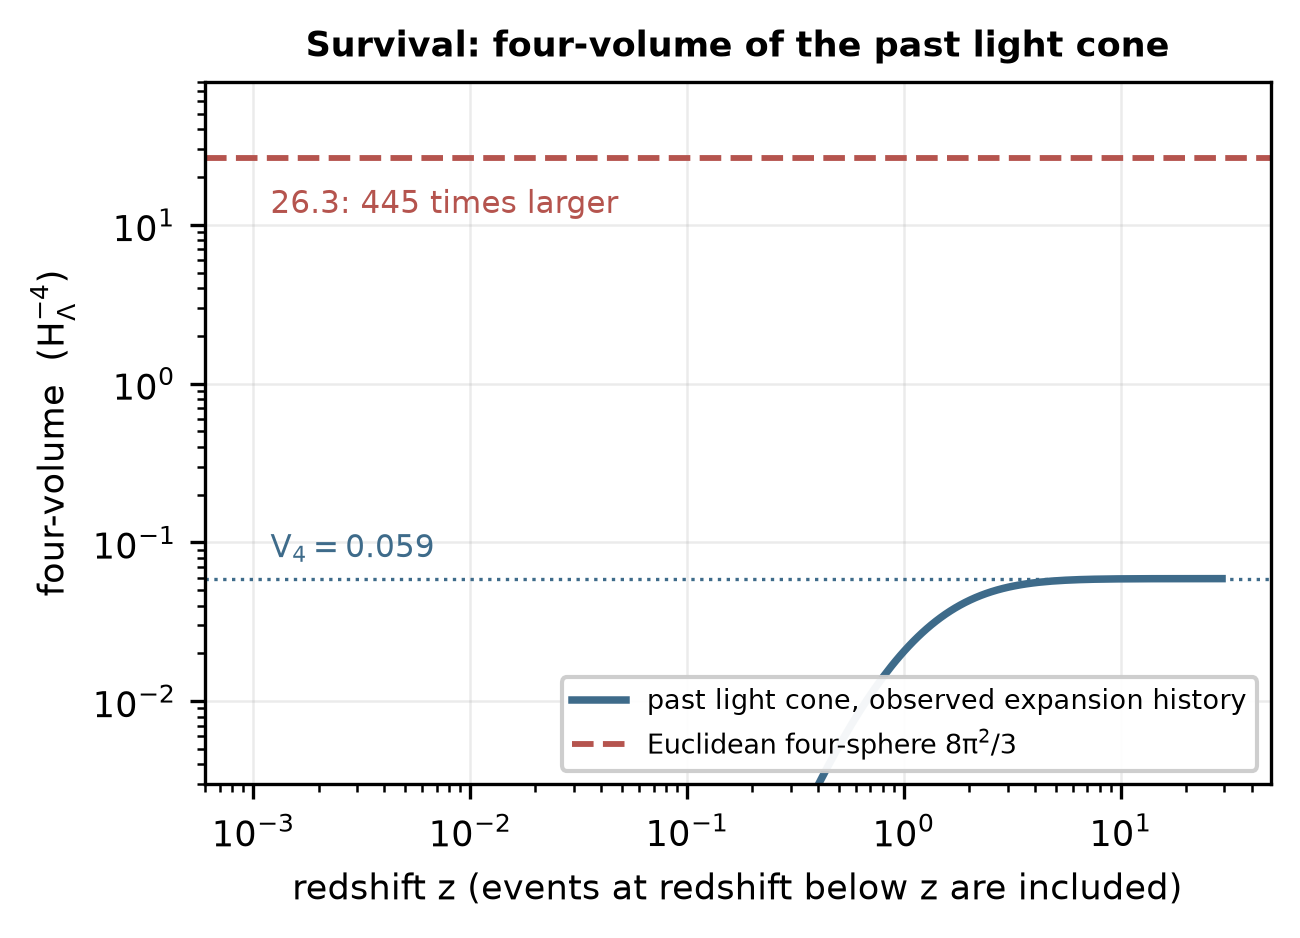
\includegraphics[width=0.59\textwidth]{../figures/fig3_survival_cone.png}\caption{Four-volume of the past light cone of the present observer, accumulated over events at redshift below $z$, for the observed expansion history, against the Euclidean four-sphere volume.}\end{figure}
The observation that no bubble has reached us is excluded at 95\% confidence if $\Gamma V_4>-\ln0.05=3.00$, that is for $\Gamma/H^4>50.7$ or $B<B_c-3.9$. This is a weak condition: it is 1334 times weaker than the Euclidean estimate ($\Gamma/H^4>0.038$), it moves the boundary of the allowed region by only $\Delta B=7.2$ out of about 287, and it bounds the future mean decay time only by $t_{\rm dec}\gtrsim8.2\times10^{7}$ yr (the formula for $t_{\rm dec}$ is used here as an order-of-magnitude statement, since $\Gamma/H^4$ is not small). Because the prior mass sits overwhelmingly at $B\ll B_c$ or $B\gg B_c$, the fraction of the prior excluded changes from 15.0\% (Euclidean estimate) to 14.8\% (Section 4.5). The criterion assumes that $\Gamma$ was constant, with the scalar in its false minimum throughout; it does not require observers to be present before the transition, and it says nothing about bubbles nucleated outside our past cone. Percolation of bubbles in de Sitter space requires a rate of order unity in Hubble units [16, 17], since otherwise the false-vacuum volume grows without bound and no wall collides with another. With the corrected survival bound this no longer conflicts with survival: the window $1\lesssim\Gamma/H^4<51$ has the width $\Delta B=3.9$ and contains 0.12\% of the prior volume (0.18\% for a percolation threshold of 0.1 and 0.05\% for 10).

\subsection{The prefactor and the validity of the semiclassical rate}
The factor $D$ is the ratio of the fluctuation determinants with the zero modes removed; methods to compute it for specific potentials exist [12, 13] and are not repeated here. It is treated as a systematic uncertainty. Because $\ln D$ enters $B_c$ additively, a change of $D$ by $n$ decades moves $B_c$ by $2.3\,n$: three decades give $\pm7$ out of $287$, six decades give $\pm14$ (5\%), and the prior mass of every regime changes by less than $10^{-3}$ over spreads of 0, 3 and 6 decades (Table 5). The semiclassical expansion is controlled by $1/B$, which is $3.5\times10^{-3}$ at $B_c$, so that higher-loop corrections change $\ln\Gamma$ by $O(1)$ and not $O(B)$, which the prefactor spread already covers. The regime in which the approximation fails is $B=O(1)$ to $O(10)$, where the wall is not thin on the scale of the field fluctuations; 0.5\% of the prior has $B<10$ and 2.5\% has $B<30$, and none of these draws survives the survival condition (all have $\Gamma/H^4\gg51$), so the failure of the semiclassical approximation affects only the excluded region and cannot change the classification of any draw that is allowed.

\subsection{The falsification diagram}
Fig. 4 maps the decay time over the $(\eta,\lambda)$ plane for $r_L=1$. The region excluded by survival and the region of effective stability ($t_{\rm dec}>10^{100}$ yr) are separated by a band: the decay time runs from the survival bound of $8.2\times10^{7}$ yr to $10^{20}$ yr within a change of $\Delta B\simeq28$ in the action and to $10^{100}$ yr within $\Delta B\simeq212$. The model is thus either excluded, or it describes a vacuum that decays on a time scale of $10^{20}$ yr or longer unless $B$ is tuned to within about $28$ of the survival bound, that is within 10\% of its value.

\begin{figure}[htbp]\centering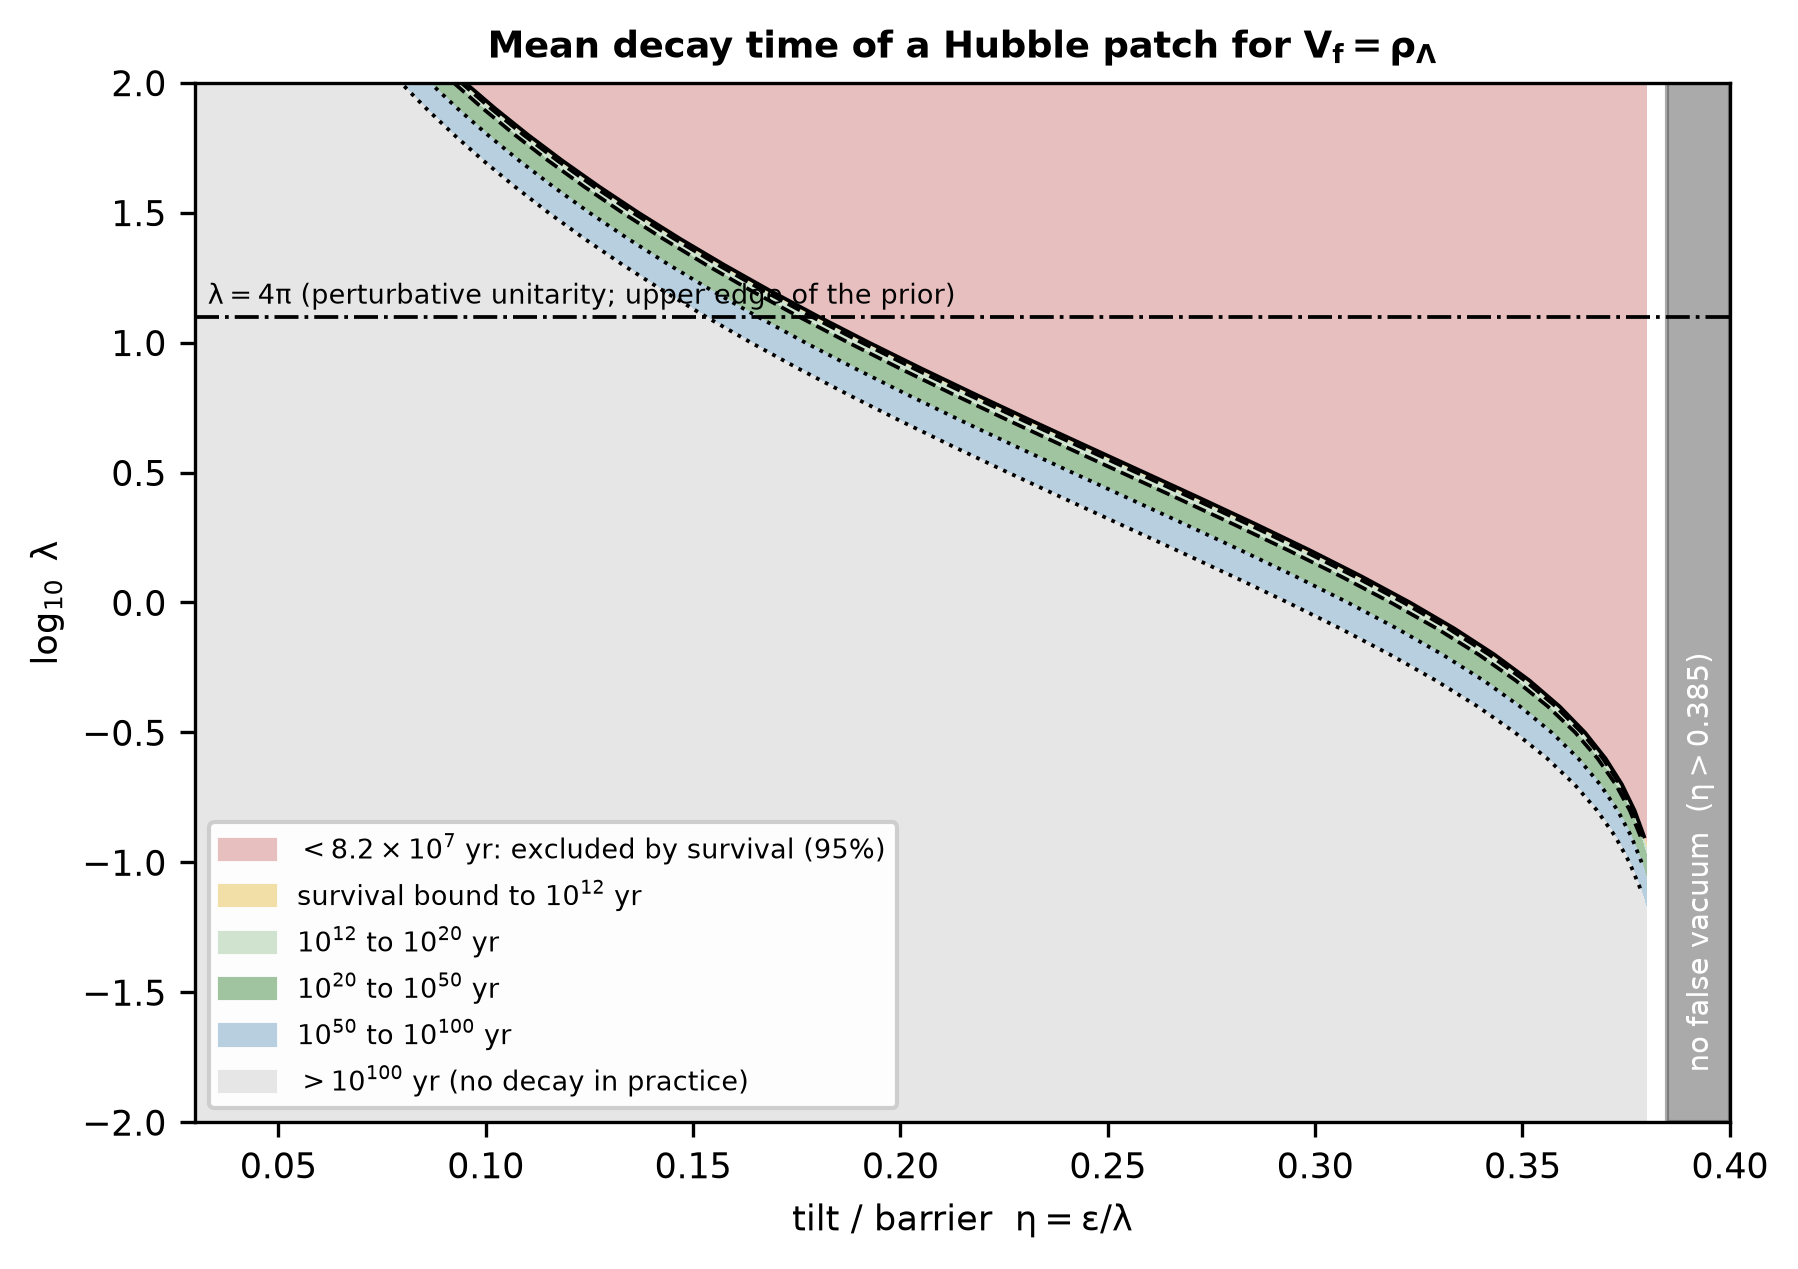
\includegraphics[width=1.00\textwidth]{../figures/fig4_falsification_diagram.png}\caption{Mean decay time of a Hubble patch in the $(\eta,\lambda)$ plane for $V_f=\rho_\Lambda$ and a Minkowski true vacuum. Contours: survival bound ($8.2\times10^{7}$ yr), $10^{12}$, $10^{20}$, $10^{50}$ and $10^{100}$ yr. The upper edge $\lambda=4\pi$ is the perturbative-unitarity limit used for the prior.}\end{figure}
\subsection{Prior-sensitivity Monte Carlo}
To quantify how much of the parameter space the window occupies, $1,000,000$ parameter sets are drawn from physically consistent priors ($\log_{10}\lambda$ uniform on $[-2,\log_{10}4\pi]$, $\eta$ uniform on $[0.03,0.38]$, $\ln D$ Gaussian with a spread of 1.5 decades; the false minimum exists for every draw) and each is converted to a rate with the interpolated numerical action. The regime fractions are given in Table 5 together with batch-means standard errors (20 batches), convergence with the number of draws (Fig. 5c) and sensitivity to the priors. 14.8\% of the prior volume lies above the survival bound, 0.77\% decays within $10^{20}$ yr, 4.8\% within $10^{100}$ yr and 80.4\% shows no decay within $10^{100}$ yr. The fractions do not depend on the prefactor and the choice of $r_L$ is likewise immaterial. They do depend on the prior range of $\lambda$ and $\eta$ (Table 5; for $\lambda\le1$ the excluded fraction falls to 2.8\%). They are therefore fractions of the stated prior, a property of the parameter space of this model and not measured probabilities, and they do not indicate how likely a transition is in our universe. $V_t<0$ would enter through $r_L=1/(1+|V_t|/V_f)<1$ and shifts $B_c$ upward by $\ln(1+|V_t|/V_f)$; the case $r_L\ge1$ is the one sampled.

\begin{table}[htbp]\centering\small
\caption{Prior mass (\%) of each regime. Decay fractions are cumulative and refer to survival-consistent draws; the last column is the fraction with no decay within $10^{100}$ yr. These are fractions of the stated prior, not probabilities for our universe.}
\begin{tabular}{llllll}
\toprule
Prior & above survival bound & decays by $10^{12}$ yr & by $10^{20}$ yr & by $10^{100}$ yr & no decay in $10^{100}$ yr \\ \midrule
baseline & 14.77 $\pm$ 0.04 & 0.269 $\pm$ 0.005 & 0.77 $\pm$ 0.01 & 4.78 $\pm$ 0.02 & 80.4 $\pm$ 0.0 \\
$\sigma_{\log D}$ = 0 & 14.74 & 0.270 & 0.76 & 4.80 & 80.5 \\
$\sigma_{\log D}$ = 3 & 14.75 & 0.257 & 0.75 & 4.79 & 80.5 \\
$\sigma_{\log D}$ = 6 & 14.74 & 0.267 & 0.76 & 4.79 & 80.5 \\
$r_L$ ~ logU(1, 10) & 14.71 & 0.264 & 0.76 & 4.80 & 80.5 \\
$\lambda$ $\le$ 1 & 2.76 & 0.122 & 0.35 & 2.50 & 94.7 \\
$\eta$ in [0.10, 0.38] & 18.45 & 0.323 & 0.95 & 5.96 & 75.6 \\
log10 $\lambda$ in [-4, 2] & 18.18 & 0.190 & 0.55 & 3.35 & 78.5 \\
\bottomrule
\end{tabular}
\end{table}
\begin{figure}[htbp]\centering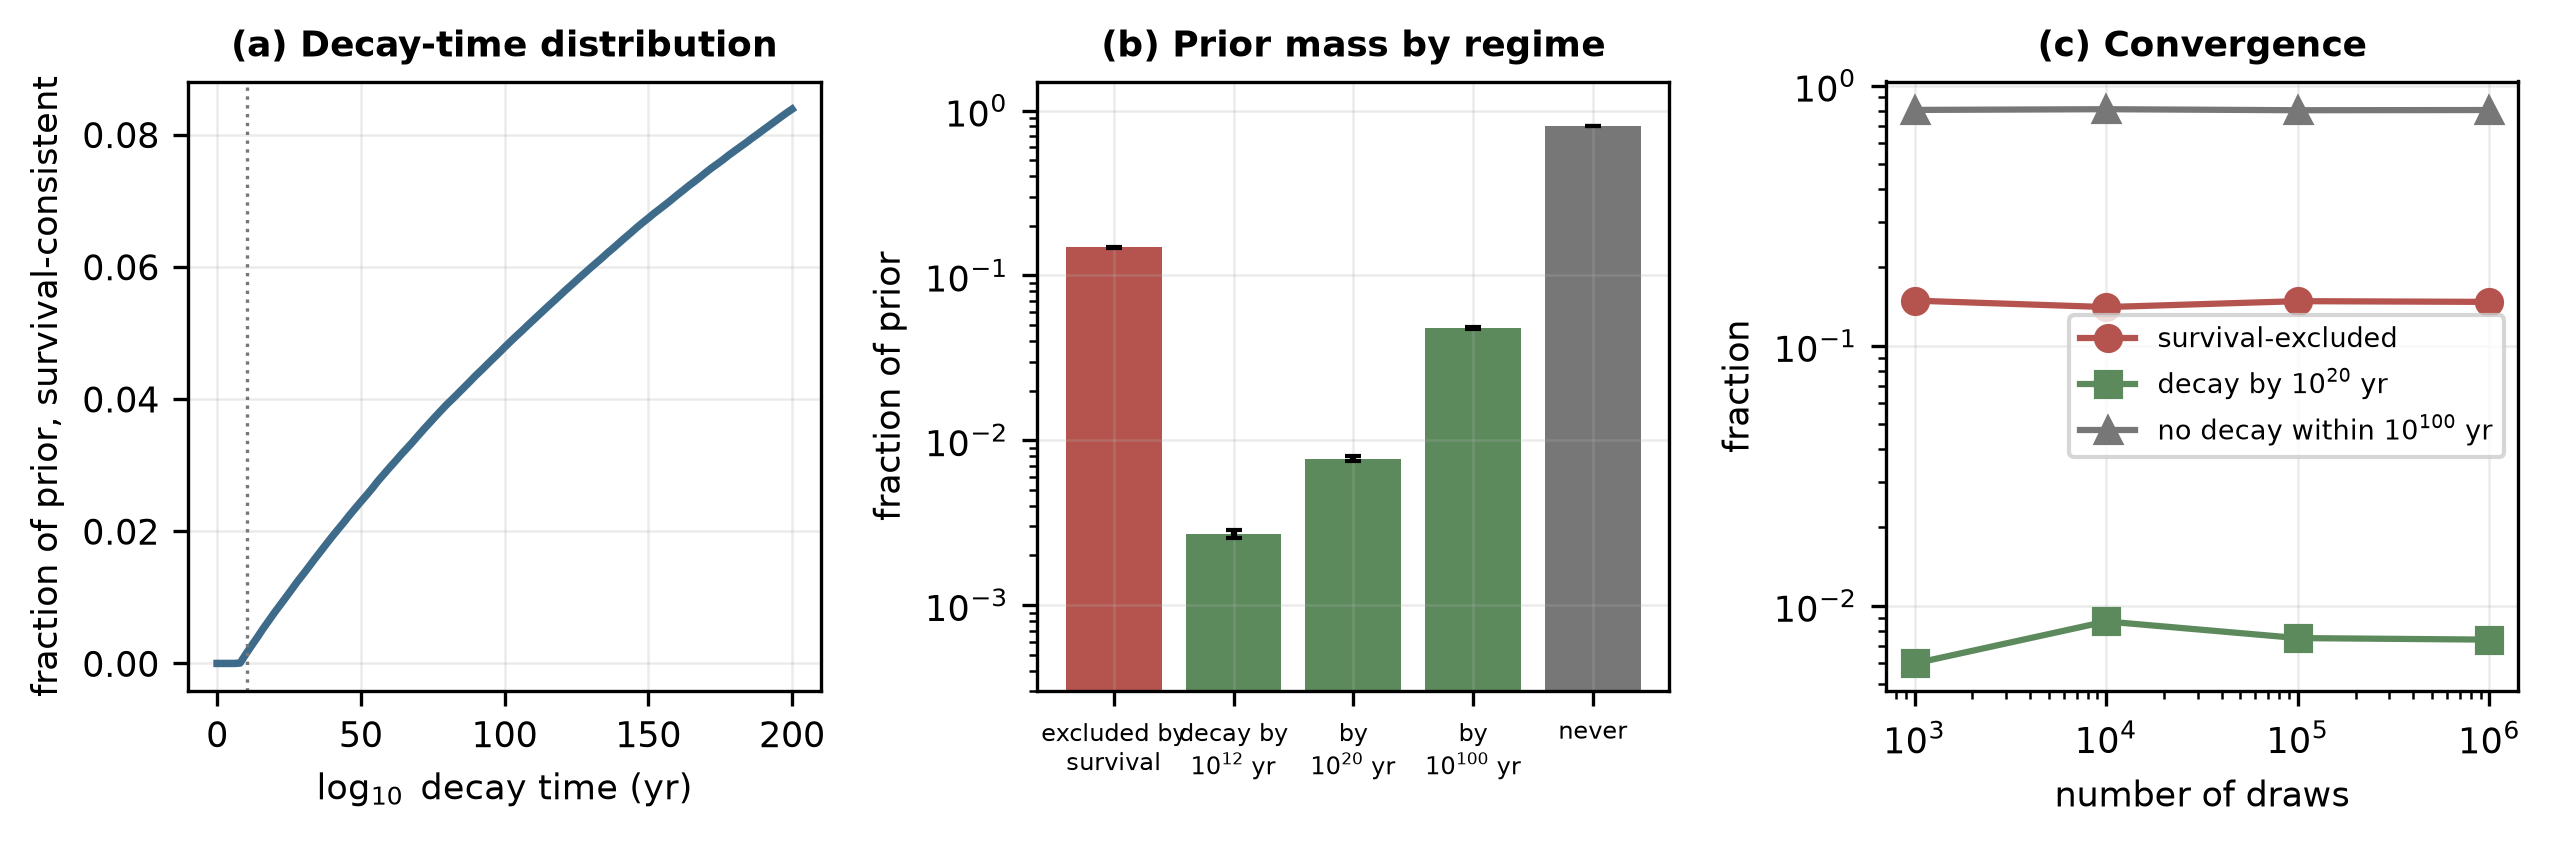
\includegraphics[width=1.00\textwidth]{../figures/fig5_monte_carlo.png}\caption{(a) Cumulative distribution of the decay time over survival-consistent draws. (b) Prior mass by regime with $3\sigma$ batch errors. (c) Convergence of the regime fractions with the number of draws.}\end{figure}
\section{What the nucleated region can become}
\subsection{Energy budget}
A thin-wall bubble of true vacuum is bounded by a wall that carries the released energy; its interior is, to leading order, the true vacuum with no excess energy to reheat. In the thick-wall regime relevant here the field at the centre of the bounce, $x_0$, lies above the true minimum, and the energy the interior can release is $\epsilon_{\rm in}\Delta V = V(x_0)-V_t$. Fig. 6c shows $\epsilon_{\rm in}$ against $\eta$: at $\eta=0.30$, $\epsilon_{\rm in}=0.018$, so 1.8\% of $\Delta V$ resides in the interior and the remainder in the wall; $\epsilon_{\rm in}$ approaches unity only near $\eta_c$, where the barrier is gone.

\subsection{Interior geometry and reheating}
The interior of a CDL bubble has open spatial slices, $ds^2=-dt^2+a(t)^2dH_3^2$ [18, 19], with the Friedmann constraint $(da/dt)^2 = 1 + a^2\rho/(3M_{\rm Pl}^2)$. Without a long inflationary stage inside the bubble (Section 5.3), the energy density is negligible against the curvature term at early times: $\alpha^2\rho \le 1.1\times10^{-61}$ in units where $H_\Lambda=1$, so the interior is a Milne universe, $a=t$. The condensate begins to oscillate at $t_0 = 1/m$ with $m = 3.61$ meV, behaves as matter and decays to radiation at a rate $\Gamma_\varphi\le m$. With $\tau=H_\Lambda t$ the radiation density has the closed form $\rho_r(\tau)=\epsilon\,\tau_0^3\,\gamma\,\tau^{-4}\int_{\tau_0}^{\tau}s\,e^{-\gamma(s-\tau_0)}ds$ in units of $V_f$, which we compare with a numerical integration of the full system (relative difference $6\times10^{-7}$). The radiation temperature is $T=(30\rho_r/\pi^2g_*)^{1/4}$ with $g_*=3.36$.

Energy conservation bounds the reheating temperature independently of the details of the decay,

\begin{equation}
T_{\rm reh}\le\left[\frac{30\,\epsilon_{\rm th}\,\epsilon_{\rm in}\Delta V}{\pi^2g_*}\right]^{1/4},\qquad \epsilon_{\rm th}\le1
\end{equation}
which for the largest release allowed when $V_t\ge0$, $\epsilon_{\rm in}\Delta V = \Delta V\le V_f=\rho_\Lambda$, gives $T_{\rm reh}\le 2.19$ meV ($25$ K), against the CMB temperature of 0.235 meV today and $4.6\times10^{8}$ times below the $\sim1$ MeV required for nucleosynthesis [32]. Equivalently, a thermal bath at 1 MeV needs an energy density $1.4\times10^{35}$ times the dark-energy density. The closed form shows that the situation is worse than the bound: the radiation temperature after its maximum falls as $T\propto1/\tau$ because the open interior keeps expanding, with $T\tau=5.46\times10^{-43}$ GeV, so $T=1$ MeV would have to occur at $t=3.0\times10^{-22}$ s, before the condensate even starts to oscillate ($t_0=1.8\times10^{-13}$ s). Table 6 gives the maximum temperature for decay rates from $\Gamma_\varphi=m$ down to $10^{-20}m$ and the temperature one Hubble time after nucleation, $\sim10^{-30}$ meV.

\begin{table}[htbp]\centering\small
\caption{Reheating of the bubble interior. $\epsilon$: fraction of $\Delta V$ in the interior; $\Gamma_\varphi/m$: decay rate of the oscillating condensate; $T_{\max}$: maximum radiation temperature; the fourth column is $T_{\max}$ over the bound of Eq. (10); the fifth is the temperature one Hubble time $1/H_\Lambda$ after nucleation; the last is $T_{\rm BBN}/T_{\max}$.}
\begin{tabular}{llllll}
\toprule
$\epsilon$ & $\Gamma_\varphi/m$ & $T_{\max}$ (meV) & $T_{\max}/T_{\rm bound}$ & $T(1/H_\Lambda)$ (meV) & $T_{\rm BBN}/T_{\max}$ \\ \midrule
1 (upper bound) & 1 & 1.2445 & 0.57 & $8.7\times10^{-31}$ & $8.0\times10^{8}$ \\
1 (upper bound) & 0.001 & 0.2318 & 0.11 & $4.1\times10^{-30}$ & $4.3\times10^{9}$ \\
1 (upper bound) & 1e-09 & 0.0073 & 0.00 & $1.3\times10^{-28}$ & $1.4\times10^{11}$ \\
1 (upper bound) & 1e-20 & 0.0000 & 0.00 & $7.3\times10^{-26}$ & $7.7\times10^{13}$ \\
0.018 ($\eta=0.30$) & 1 & 0.4558 & 0.57 & $3.2\times10^{-31}$ & $2.2\times10^{9}$ \\
0.018 ($\eta=0.30$) & 0.001 & 0.0849 & 0.11 & $1.5\times10^{-30}$ & $1.2\times10^{10}$ \\
0.018 ($\eta=0.30$) & 1e-09 & 0.0027 & 0.00 & $4.7\times10^{-29}$ & $3.7\times10^{11}$ \\
0.018 ($\eta=0.30$) & 1e-20 & 0.0000 & 0.00 & $2.7\times10^{-26}$ & $2.1\times10^{14}$ \\
\bottomrule
\end{tabular}
\end{table}
\begin{figure}[htbp]\centering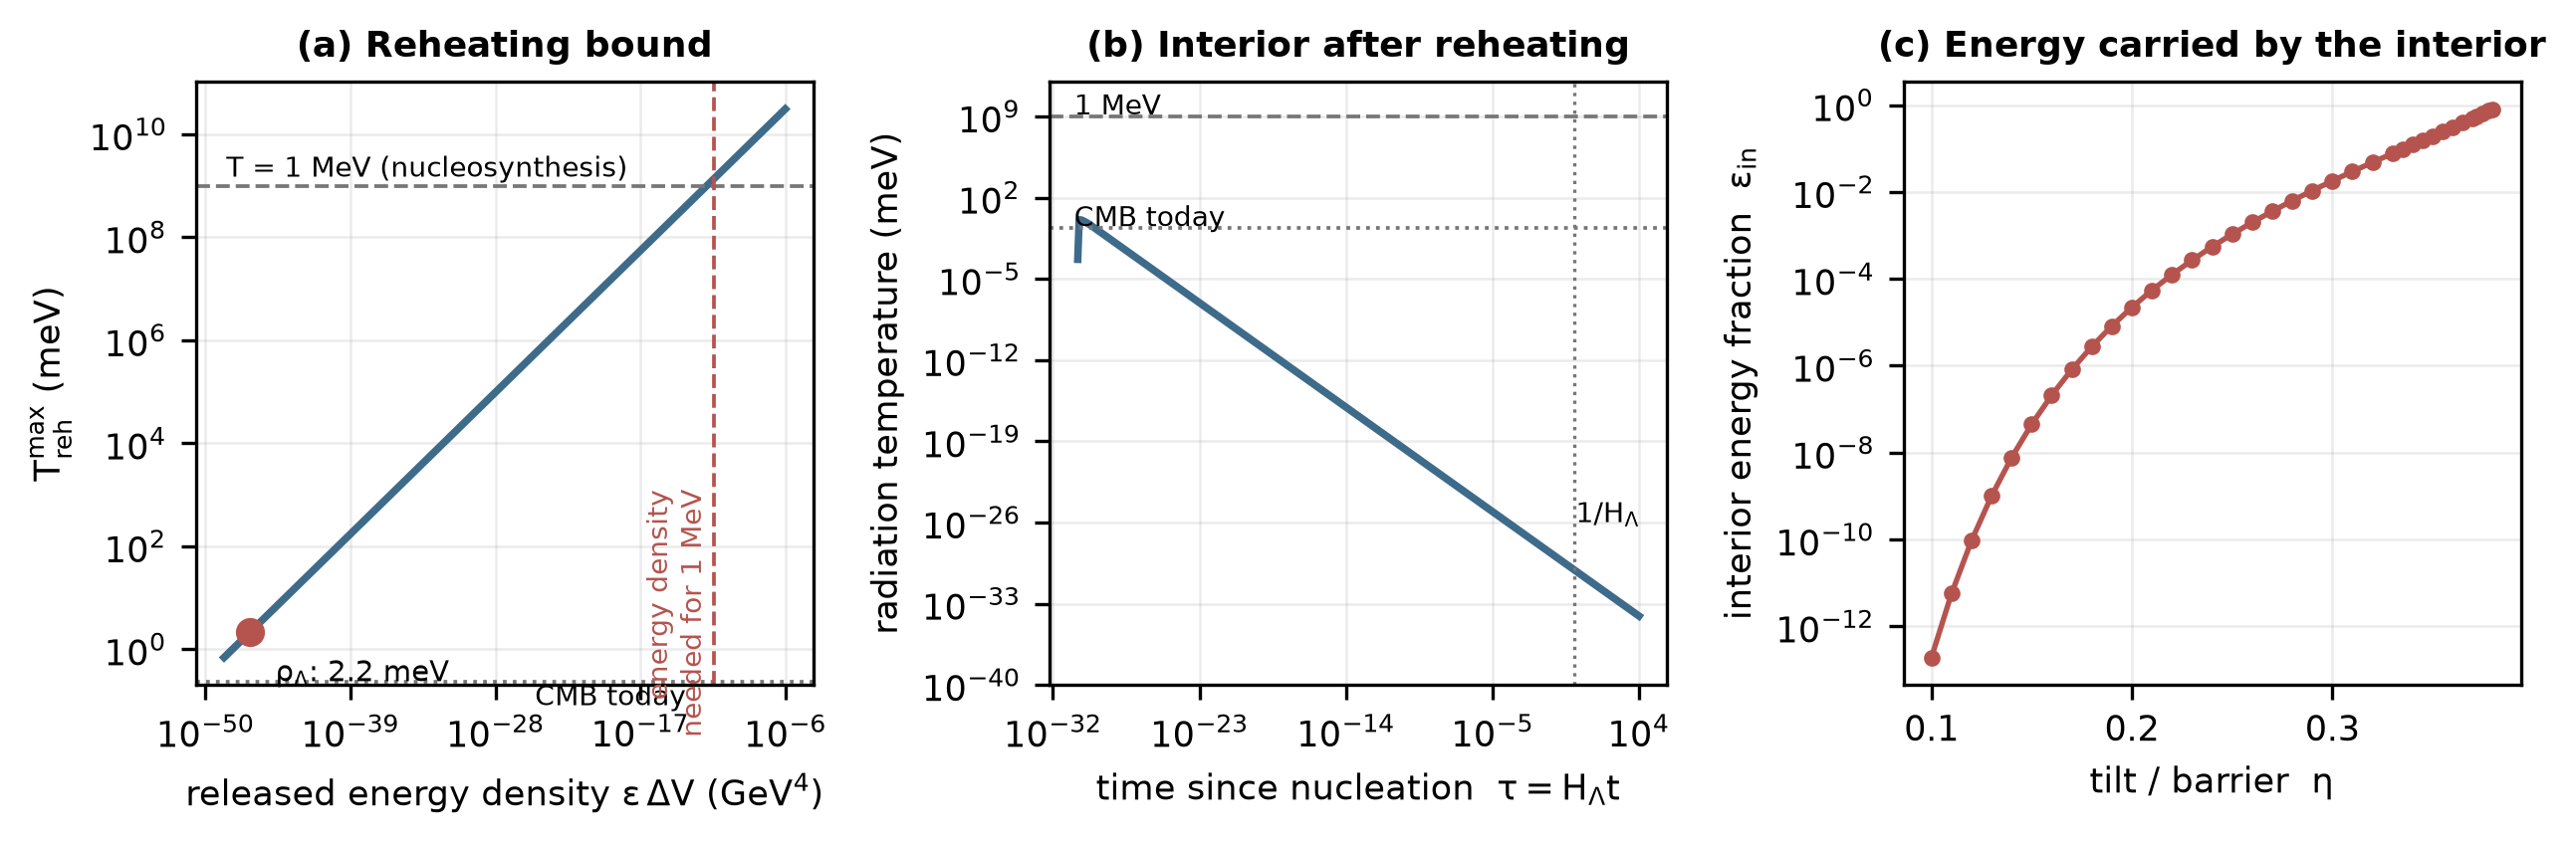
\includegraphics[width=1.00\textwidth]{../figures/fig6_reheating_interior.png}\caption{(a) Maximum reheating temperature against the released energy density; the dark-energy density gives about 2 meV, far below the energy density needed for 1 MeV. (b) Temperature of the open interior after reheating ($\Gamma_\varphi=m$): the radiation cools as $1/t$ and never approaches nucleosynthesis. (c) Fraction of $\Delta V$ carried by the interior against the tilt.}\end{figure}
\subsection{Scope of the bound: what is excluded by the model and what only by energy conservation}
The bound of Eq. (10) is a statement about a locally homogeneous conversion of a vacuum-energy difference that does not exceed the dark-energy density. It is not a universal prohibition on high-temperature bubble interiors, and it is stated here with its assumptions: (A1) one real scalar field minimally coupled to gravity, with the potential of Section 2; (A2) the false-vacuum energy is the observed dark energy; (A3) the interior is homogeneous and isotropic on open slices; (A4) no inflationary stage inside the bubble; (A5) all energy densities are sub-Planckian. Models that violate one of these need a separate analysis. Table 7 lists the possible additional energy sources and says which of them the model excludes by more than energy conservation.

The geometric argument is the following. In the open slicing the curvature parameter $Y\equiv a^2\rho/(3M_{\rm Pl}^2)$ obeys $(da/dt)^2=1+Y$. A hot big bang at nucleosynthesis needs $Y\sim1$: in standard radiation domination $Ht=1/2$, that is $\rho t^2=3M_{\rm Pl}^2/4$. In the curvature-dominated phase $a=t$ and $Y=\rho t^2/(3M_{\rm Pl}^2)$ can only decrease, as $1/t$ for matter and $1/t^2$ for radiation, unless the interior inflates. The energy density of the condensate and its decay products obeys the envelope

\begin{equation}
\rho(t)\le\epsilon\,\Delta V\,(mt)^{-3}\quad(t>t_0=1/m),\qquad Y(t_0)=\frac{\epsilon\,\Delta V}{3M_{\rm Pl}^2m^2}
\end{equation}
because matter dilutes more slowly than radiation and decay only moves energy from the slower to the faster component (checked against the closed form to machine precision, check V17). The mass at the true minimum is $m=\kappa_m\Delta V^{1/4}$ with $\kappa_m=\lambda^{1/4}[(3x_t^2-1)/2]^{1/2}\delta^{-1/4}$, which lies between 0.50 and 4.1 over the whole prior, so $Y(t_0)=c\sqrt{\Delta V}/M_{\rm Pl}^2$ is tiny for any sub-Planckian energy: $Y(t_0)=2.0\times10^{-63}$ at $\Delta V=V_f$, and $Y(t_0)=1$ would need $\Delta V/M_{\rm Pl}^4=1.8\times10^{5}$ at the benchmark, which is super-Planckian. Therefore, for any $\Delta V$ below the Planck scale, the interior is a Milne universe at all times, $Y$ never approaches unity (Fig. 7), and the energy density at one second after nucleation cannot exceed $\epsilon\Delta V/(m\cdot1\,{\rm s})^3$. Requiring $\rho(1\ {\rm s})\ge\rho_{\rm BBN}=(\pi^2g_*/30)(1\ {\rm MeV})^4$ ($g_*=10.75$) demands $\Delta V^{1/4}\ge5.1\times10^{61}$ GeV, that is 42, 43 and 45 orders of magnitude above the Planck mass (for the smallest $\kappa_m$ in the prior, the benchmark and the largest). For the dark energy the envelope gives $\rho(1\ {\rm s})=4.4\times10^{-74}\,\rho_{\rm BBN}$.

\begin{figure}[htbp]\centering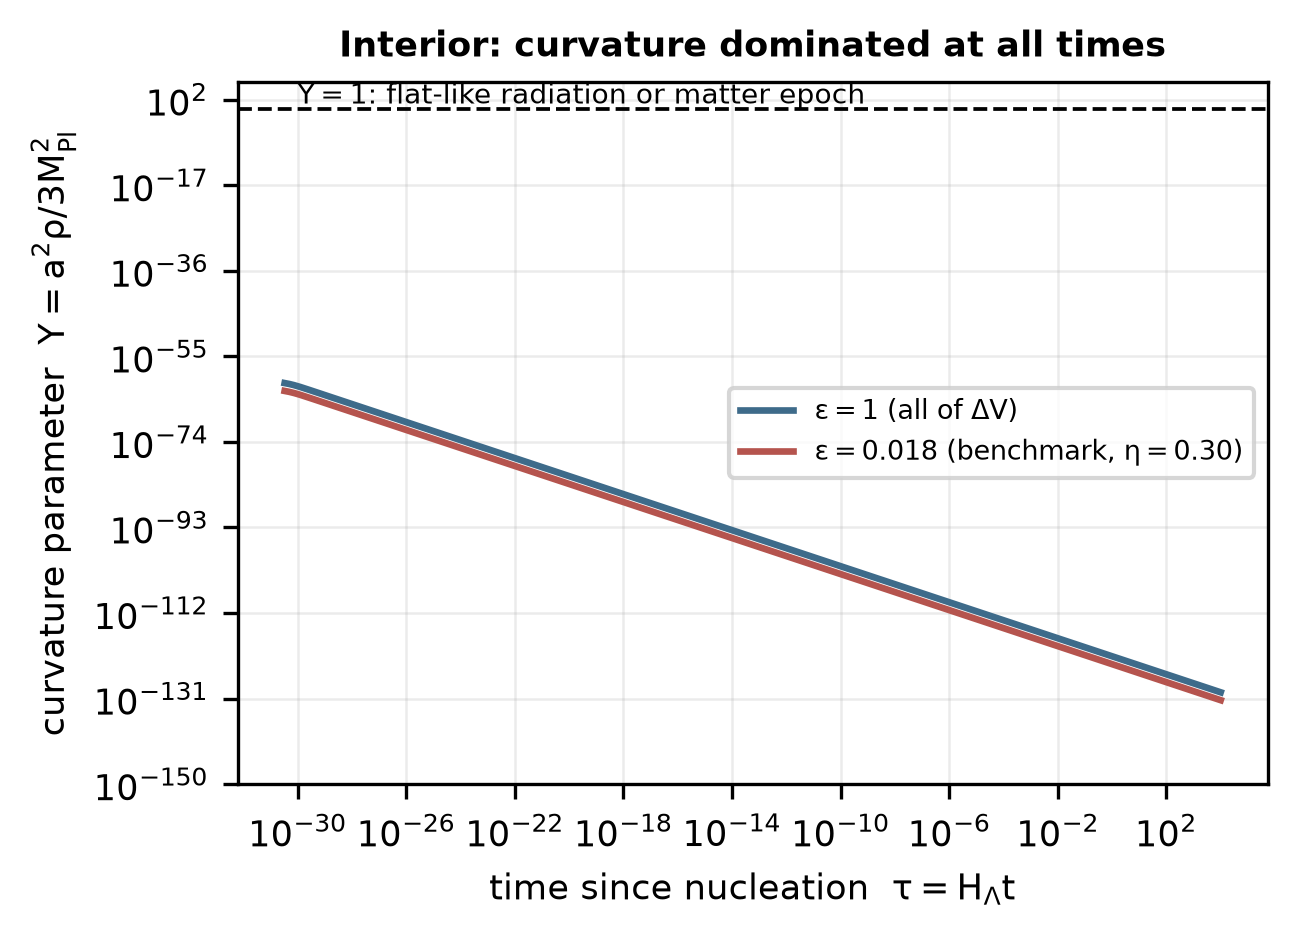
\includegraphics[width=0.59\textwidth]{../figures/fig7_curvature_interior.png}\caption{Curvature parameter $Y=a^2\rho/3M_{\rm Pl}^2$ of the bubble interior against the time since nucleation for $\Gamma_\varphi=m$. A flat-like radiation- or matter-dominated epoch needs $Y\sim1$; the interior starts at $Y\sim10^{-63}$ and moves away from it.}\end{figure}
\begin{table}[htbp]\centering\small
\caption{Energy sources and assumptions behind the reheating bound, and what excludes each.}
\begin{tabular}{>{\raggedright\arraybackslash}p{0.255\dimexpr\textwidth-6\tabcolsep\relax}>{\raggedright\arraybackslash}p{0.373\dimexpr\textwidth-6\tabcolsep\relax}>{\raggedright\arraybackslash}p{0.373\dimexpr\textwidth-6\tabcolsep\relax}}
\toprule
Source or assumption & What bounds it & Quantitative statement \\ \midrule
Released vacuum energy, $V_t\ge0$ & energy conservation, $\Delta V\le V_f$ & $T_{\rm reh}\le2.19$ meV \\
Wall energy $(1-\epsilon_{\rm in})\Delta V$ & already counted in $\Delta V$; collisions redistribute it & benchmark: 98\% of $\Delta V$ in the wall; the total is unchanged \\
Deeper true vacuum, $V_t<0$ (anti-de Sitter) & geometry: crunch at $t_c=\pi\sqrt3M_{\rm Pl}/\sqrt{|V_t|}$ and the curvature envelope & $T_{\max}=1$ MeV needs $|V_t|=1.4\times10^{35}\,V_f$ and a crunch after 4.6 s; a life of 13.8 Gyr needs $|V_t|\le15.7\,V_f$ and $T\le4.4$ meV \\
Interior inflation & the potential has no plateau above $V_f$; field range $\Delta\varphi/M_{\rm Pl}\sim10^{-30}$ & at most $9.3\times10^{-62}$ e-folds (largest over four tilts) \\
Larger parent scale ($V_f\gg\rho_\Lambda$) & geometry: the envelope $\rho\le\epsilon\Delta V(mt)^{-3}$ & $\rho(1\ {\rm s})\ge\rho_{\rm BBN}$ needs $\Delta V^{1/4}$ 42 to 45 orders above $M_{\rm Pl}$ \\
Extra reservoir (other fields, radiation) & not part of the model; subject to the same curvature constraint & $Y\sim1$ at $t=1/m$ needs $\rho_x=9.1\times10^{60}\,\Delta V$ \\
Inhomogeneity, bubble collisions & not included (A3); total energy is bounded by $\Delta V$ & local concentration possible; the average is unchanged \\
\bottomrule
\end{tabular}
\end{table}
Three points follow. First, the anti-de Sitter case shows that energy conservation alone is not sufficient: a very deep true vacuum releases enough energy for 1 MeV, but its open interior then collapses within seconds, and the longest-lived interior has $T\lesssim4$ meV. Second, the geometric statement is independent of the energy scale and of the value of $V_f$, and therefore covers an additional reservoir too: it cannot raise $Y$ above the curvature bound unless its energy density exceeds $\Delta V$ by $9.1\times10^{60}$. Third, the escape routes are exactly those the model lacks: a long inflationary stage inside the bubble, a parent energy scale close to the Planck scale, or an additional mechanism that raises $Y$ at $t_0$. A successful cosmology would have to lie in that outside class.

\subsection{Other fates and the singularity question}
If the true vacuum has negative energy ($V_t<0$) the open interior collapses to a singularity in a finite time, $\tau_c = \pi/\sqrt{|V_t|/V_f}$: $|V_t|=0.01\,V_f$: 547 Gyr; $|V_t|=0.1\,V_f$: 173 Gyr; $|V_t|=1\,V_f$: 55 Gyr; $|V_t|=10\,V_f$: 17 Gyr. A decay to a de Sitter vacuum with $V_t>0$ leaves the interior with an accelerating phase and no radiation epoch. Only $V_t\simeq0$ leaves a regular, expanding, but empty interior. No case yields a nonsingular bounce from the parent geometry: the bubble is a region of the parent de Sitter space, causally connected to it, and the Milne interior is geodesically complete only because it has no matter.

\section{Matter dilution and decoherence as a trigger}
The original motivation for a late-time transition was that dilution of matter reduces environmental decoherence and thereby permits a macroscopic quantum transition. In the baseline model nothing of the kind appears: the potential $V(\varphi)$, hence $B$, does not depend on the matter density, and the Gibbons--Hawking temperature $T_H=H/2\pi=1.9\times10^{-43}$ GeV [33] is $6\times10^{-32}$ of the field scale; thermal-type corrections to $B$ are of relative size $\sim g\,(\kappa\simeq3.5)$, that is $10^{-59}$ (Section 3.4). A dependence on matter must be introduced by a coupling, and a conclusion that held only for one coupling would be weak. The requirement can be stated without choosing one.

Any coupling of non-relativistic matter of mass $m_{\rm mat}(\varphi)$ adds $\rho_m\ln m_{\rm mat}(\varphi)$ to the effective potential, so that the energy difference between the vacua changes by $\rho_m\,\Delta\ln m$, where $\Delta\ln m$ is the fractional change of the matter mass between the two field values and $\rho_m=(\Omega_m/\Omega_\Lambda)V_f$ today. Write $\varepsilon_m\equiv\rho_m\Delta\ln m/\Delta V$ for the relative shift. To first order in the tilt shift $\Delta\eta$,

\begin{equation}
\frac{\Delta\eta}{\eta}=\frac{2\,\delta(\eta)}{\eta\,(x_f-x_t)}\,\varepsilon_m,\qquad \Delta B=B\left|\frac{d\ln b}{d\ln\eta}\right|\frac{\Delta\eta}{\eta}
\end{equation}
with $\delta(\eta)=\Delta V/(\lambda f^4)$ of Eq. (3). A change of the rate by a factor $e$ needs $\Delta B=1$; moving a benchmark from $B=441$ to the critical action $B_c=287$ needs $\Delta B=154$ ($\Delta B=13.7$ for $\eta=0.32$). With $|d\ln b/d\ln\eta|=5.5$ at $\eta=0.30$ this gives $\Delta\ln m=8.9\times10^{-4}$ and $1.4\times10^{-1}$ respectively: the matter mass must differ by between about $0.1\%$ and $10\%$ between the two vacua. Table 8 translates this to specific couplings.

\begin{table}[htbp]\centering\small
\caption{Requirement on a matter coupling that changes the rate by a factor $e$ (left end) or moves the benchmark into the reset window (right end).}
\begin{tabular}{>{\raggedright\arraybackslash}p{0.236\dimexpr\textwidth-6\tabcolsep\relax}>{\raggedright\arraybackslash}p{0.382\dimexpr\textwidth-6\tabcolsep\relax}>{\raggedright\arraybackslash}p{0.382\dimexpr\textwidth-6\tabcolsep\relax}}
\toprule
Coupling & Requirement & Comment \\ \midrule
General & $\Delta\ln m\ge8.9\times10^{-4}$ to $1.4\times10^{-1}$ & independent of the coupling function; $\eta=0.30$ \\
Linear, $m=m_0e^{\beta\varphi/M_{\rm Pl}}$ & $\beta\ge3.7\times10^{26}$ to $5.7\times10^{28}$ (for $\eta=0.32$: $4.7\times10^{26}$ to $6.4\times10^{27}$) & $\Delta\varphi/M_{\rm Pl}=2.4\times10^{-30}$; unscreened tests restrict $\beta\lesssim O(1)$; screening (chameleon type) lowers the local coupling, not the cosmological one [25] \\
Quadratic, $m=m_0(1+\varphi^2/2\Lambda_q^2)$ & $\Lambda_q\le58$ to $5$ meV ($\eta=0.30$) & $f=3.0$ meV, so $\Lambda_q\sim(2$--$20)f$: a new interaction at the scale of the potential; symmetron-type screening [26] can hide it in dense environments \\
Density-dependent effective potential & same $\Delta\ln m$ & the model is then specified by $\rho_m F(\varphi)$ with $F$ changing by that amount across $\Delta\varphi$ \\
\bottomrule
\end{tabular}
\end{table}
The conclusion is therefore conditional. For the simplest linear coupling the required strength lies $26$ to $28$ orders of magnitude above what unscreened laboratory and solar-system tests allow. Quadratic or screened couplings are not excluded by this paper: they evade local tests by construction, but they are tuned, because they require a coupling scale of the same size as the dark-energy potential and a mass change of at least $0.1\%$ of the matter between vacua. The dilution of matter can act as a trigger only through such an added, tuned structure, not through the framework itself. A noise-assisted mechanism would need an explicit open-system influence functional and a calculated change of the tunneling exponent, which is not assumed here.

\section{Consistency conditions and falsification tests}
A model of this class must satisfy internal consistency conditions, which are mathematical or follow from the framework, and it can be confronted with observational tests. The two are kept apart because failing the first means the model is ill-defined, while failing the second means that it is disfavored by data. All are computed in this paper and can be recomputed for a different potential with the supplied code.

\subsection{Internal consistency conditions}
\begin{itemize}\item C1 (existence). A metastable minimum requires $\eta<\eta_c=0.385$; for larger tilt there is nothing to decay.
\item C2 (semiclassical validity). The loop expansion parameter $1/B$ must be small. All draws with $B<30$ (2.5\% of the prior) have rates far above the survival bound, so the classification of allowed draws is unaffected (Section 4.3).
\item C3 (negative mode and flat limit). The bounce has one negative mode and gravity enters as an $O(g)$ perturbation, $g\sim10^{-60}$ (Section 3.3).
\item C4 (energy). With $V_t\ge0$ the released energy density cannot exceed $\rho_\Lambda$, so $T_{\rm reh}\le2.2$ meV; with $V_t<0$ the interior crunches (Section 5.3).
\item C5 (geometry). For any sub-Planckian energy the open interior stays curvature dominated, $Y(t)\le Y(t_0)=2.0\times10^{-63}$, unless it inflates; the single-field potential gives at most $9.3\times10^{-62}$ e-folds (Section 5.3).
\item C6 (percolation). A global transition requires $\Gamma/H^4=O(1)$ or larger, a window of width $\Delta B=3.9$ below the survival bound that holds 0.12\% of the prior volume.
\end{itemize}
\subsection{Observational tests}
\begin{itemize}\item O1 (survival). The absence of a bubble in our past light cone requires $\Gamma V_4<3.0$, i.e. $\Gamma/H^4<51$ at 95\% confidence, which excludes 15\% of the prior volume of the benchmark family and constrains the future mean decay time only to $t_{\rm dec}\gtrsim8.2\times10^{7}$ yr.
\item O2 (reset window). A transition on cosmological time scales requires $B_c\lesssim B\lesssim B_c+28$ for decay within $10^{20}$ yr; this holds for 0.77\% of the prior volume. An action above $B_c+212$ puts the decay beyond $10^{100}$ yr.
\item O3 (hot epoch). A hot universe in the nucleated region requires $\rho_{\rm reh}\gtrsim(1\ \mathrm{MeV})^4$, which is $1.4\times10^{35}$ times the dark-energy density; the bound of Section 5 excludes it for decay of the present dark energy in this framework.
\item O4 (trigger). Matter dilution as the trigger needs $\Delta\ln m\gtrsim10^{-3}$ between the vacua, a linear coupling of $\beta\sim10^{26}$--$10^{29}$ or a screened coupling at a scale of tens of meV (Section 6), which local gravity and fifth-force tests can probe if the screening is incomplete.
\item O5 (signals). A solitary transition produces no signal in our patch; bubble collisions [20, 23, 24] require a population and $\Gamma/H^4=O(1)$ (C6). The vacuum is indistinguishable from a cosmological constant ($w=-1$) until it decays. A measured evolution of the dark energy, which recent baryon-acoustic-oscillation analyses combined with the CMB and supernovae prefer at the level of a few standard deviations depending on the supernova sample [34], would favor a rolling field and not a metastable vacuum. No observational discriminant of the cyclic reset is available from this model.
\end{itemize}
A transition producing a successful cosmology would have to lie outside the class studied here. It would need a parent vacuum energy of at least $\sim10^{34}\rho_\Lambda$ (an earlier, higher-energy phase of the universe rather than the present one) and, by Section 5.3, a post-nucleation region that inflates before it reheats, so that the curvature term and the horizon are handled, and a mechanism to restore the high-energy parent from the late universe. The cyclic models that have been constructed provide such mechanisms by other means [4, 5]; this paper shows that tunneling of the present dark energy does not.

\section{Discussion and limitations}
\begin{itemize}\item A single scalar field and a quartic-tilt potential are used. Other potentials change $b(\eta)$ and the interior energy fraction, but not the scales: the rate depends on the combination $M_{\rm Pl}^4/V_f$ and the interior energy on $V_f$, both fixed by the data, so O1, O3 and the geometric argument of Section 5.3 are generic.
\item The one-loop prefactor is a systematic uncertainty, not a result; the conclusions are insensitive to it over six decades (Section 4.3).
\item The decay is treated as a flat-space process because $g\sim10^{-60}$; the gravitational code is validated against analytic limits and used for the map of the regime in which gravity matters, which the dark-energy scale excludes.
\item The survival criterion assumes a constant rate and a false vacuum throughout the history of the observed universe; a field that evolved or was thermally affected in the early universe would change the early part of the cone, which carries a small part of $V_4$.
\item The interior evolution assumes a homogeneous open slicing and a perturbative decay of the condensate to radiation; bubble-wall collisions can concentrate energy locally, but the average energy density is bounded by $\Delta V$ (Table 7).
\item Up-tunneling from the false to a higher vacuum, the decay of the true vacuum in curved space [35], thermal activation of the Hawking--Moss type [36] and decays of the present vacuum into other vacua are not considered.
\item The priors of the Monte Carlo are documented assumptions, not measurements; the regime fractions describe the sample space of the model, not the probability of a transition in our universe.
\item The matter-coupling analysis is first order in the tilt shift and does not simulate any specific screened model.
\end{itemize}
\section{Conclusions}
A late-time false-vacuum transition of the present dark energy is a well-defined calculation, and for the explicit potential studied it can be done to a stated precision. The result is a set of boundaries. The decay is a flat-space process controlled by the action $B=b(\eta)/\lambda$, which must lie near $B_c\approx287$ for the transition to be neither excluded nor effectively absent; with the survival of the present vacuum evaluated on the past light cone, the bound is weak ($\Gamma/H^4<51$) and the window is set by the action itself, with 0.8\% of the stated prior volume decaying within $10^{20}$ yr. The interior of a nucleated region carries at most the dark-energy density, reheats to at most $2.2$ meV and cools as $1/t$ in a curvature-dominated open universe; this conclusion rests on geometry and not on energy conservation alone, and it holds for any sub-Planckian parent energy. A trigger by matter dilution needs a change of the matter mass between the vacua of at least $0.1\%$. The cyclic-reset hypothesis, in the form tested, is therefore not supported, and the framework identifies what would have to change.

\section*{Declarations}
\noindent\textbf{Funding.} This research received no specific grant from funding agencies in the public, commercial, or not-for-profit sectors.

\noindent\textbf{Conflict of interest.} The author declares no competing interests.

\noindent\textbf{Ethics approval, consent to participate, consent for publication.} Not applicable.

\noindent\textbf{Data availability.} The data underlying every figure and table (bounce tables, error budget, survival calculation, falsification map, Monte Carlo summary, interior evolution, scope and coupling estimates, verification results) are deposited with the code at https://github.com/sandlerleon/late-time-vacuum-decay and archived at https://doi.org/10.5281/zenodo.23751350.

\noindent\textbf{Code availability.} All code (Python, NumPy, SciPy, Matplotlib) is released under the MIT licence at https://github.com/sandlerleon/late-time-vacuum-decay, archived at https://doi.org/10.5281/zenodo.23751350. Running the scripts in the stated order regenerates every number in this paper, and verify.py runs 18 executable checks. The manuscript is archived at https://doi.org/10.5281/zenodo.23751349.

\noindent\textbf{Authors' contributions.} L.S.: conceptualization, methodology, software, formal analysis, investigation, visualization, writing.

\noindent\textbf{Use of generative AI.} During the preparation of this work the author used Claude (Anthropic) to assist with the design of the numerical analysis, writing of the code, literature checking and drafting. The author reviewed and edited the content, checked the code against analytic limits and executable tests, verified the cited references, and takes full responsibility for the publication. No AI tool is an author.

\section*{References}
\noindent\hangindent=1.5em [1] S. Coleman, F. De Luccia, Gravitational effects on and of vacuum decay. Phys. Rev. D 21, 3305--3315 (1980). https://doi.org/10.1103/PhysRevD.21.3305\par
\noindent\hangindent=1.5em [2] R. Penrose, Cycles of Time: An Extraordinary New View of the Universe. Bodley Head, London (2010).\par
\noindent\hangindent=1.5em [3] M. Gasperini, G. Veneziano, The pre-big bang scenario in string cosmology. Phys. Rep. 373, 1--212 (2003). https://doi.org/10.1016/S0370-1573(02)00389-7\par
\noindent\hangindent=1.5em [4] P.J. Steinhardt, N. Turok, A cyclic model of the universe. Science 296, 1436--1439 (2002). https://doi.org/10.1126/science.1070462\par
\noindent\hangindent=1.5em [5] A. Ijjas, P.J. Steinhardt, Bouncing cosmology made simple. Class. Quantum Grav. 35, 135004 (2018). https://doi.org/10.1088/1361-6382/aac482\par
\noindent\hangindent=1.5em [6] S. Coleman, Fate of the false vacuum: Semiclassical theory. Phys. Rev. D 15, 2929--2936 (1977). https://doi.org/10.1103/PhysRevD.15.2929\par
\noindent\hangindent=1.5em [7] C.G. Callan, S. Coleman, Fate of the false vacuum. II. First quantum corrections. Phys. Rev. D 16, 1762--1768 (1977). https://doi.org/10.1103/PhysRevD.16.1762\par
\noindent\hangindent=1.5em [8] S.W. Hawking, I.G. Moss, Supercooled phase transitions in the very early universe. Phys. Lett. B 110, 35--38 (1982). https://doi.org/10.1016/0370-2693(82)90946-7\par
\noindent\hangindent=1.5em [9] S. Parke, Gravity and the decay of the false vacuum. Phys. Lett. B 121, 313--315 (1983). https://doi.org/10.1016/0370-2693(83)91376-X\par
\noindent\hangindent=1.5em [10] R.A. Jensen, P.J. Steinhardt, Bubble nucleation and the Coleman--Weinberg model. Nucl. Phys. B 237, 176--188 (1984). https://doi.org/10.1016/0550-3213(84)90021-X\par
\noindent\hangindent=1.5em [11] T. Hackworth, E.J. Weinberg, Oscillating bounce solutions and vacuum tunneling in de Sitter spacetime. Phys. Rev. D 71, 044014 (2005). https://doi.org/10.1103/PhysRevD.71.044014\par
\noindent\hangindent=1.5em [12] G.V. Dunne, H. Min, Beyond the thin-wall approximation: Precise numerical computation of prefactors in false vacuum decay. Phys. Rev. D 72, 125004 (2005). https://doi.org/10.1103/PhysRevD.72.125004\par
\noindent\hangindent=1.5em [13] A. Andreassen, W. Frost, M.D. Schwartz, Scale-invariant instantons and the complete lifetime of the standard model. Phys. Rev. D 97, 056006 (2018). https://doi.org/10.1103/PhysRevD.97.056006\par
\noindent\hangindent=1.5em [14] G. Isidori, G. Ridolfi, A. Strumia, On the metastability of the Standard Model vacuum. Nucl. Phys. B 609, 387--409 (2001). https://doi.org/10.1016/S0550-3213(01)00302-9\par
\noindent\hangindent=1.5em [15] J.R. Espinosa, G.F. Giudice, A. Riotto, Cosmological implications of the Higgs mass measurement. J. Cosmol. Astropart. Phys. 2008(05), 002 (2008). https://doi.org/10.1088/1475-7516/2008/05/002\par
\noindent\hangindent=1.5em [16] A.H. Guth, E.J. Weinberg, Could the universe have recovered from a slow first-order phase transition? Nucl. Phys. B 212, 321--364 (1983). https://doi.org/10.1016/0550-3213(83)90307-3\par
\noindent\hangindent=1.5em [17] M.S. Turner, E.J. Weinberg, L.M. Widrow, Bubble nucleation in first-order inflation and other cosmological phase transitions. Phys. Rev. D 46, 2384--2403 (1992). https://doi.org/10.1103/PhysRevD.46.2384\par
\noindent\hangindent=1.5em [18] J.R. Gott III, Creation of open universes from de Sitter space. Nature 295, 304--307 (1982). https://doi.org/10.1038/295304a0\par
\noindent\hangindent=1.5em [19] M. Bucher, A.S. Goldhaber, N. Turok, Open universe from inflation. Phys. Rev. D 52, 3314--3337 (1995). https://doi.org/10.1103/PhysRevD.52.3314\par
\noindent\hangindent=1.5em [20] B. Freivogel, M. Kleban, M. Rodriguez Martinez, L. Susskind, Observational consequences of a landscape. J. High Energy Phys. 2006(03), 039 (2006). https://doi.org/10.1088/1126-6708/2006/03/039\par
\noindent\hangindent=1.5em [21] R. Bousso, J. Polchinski, Quantization of four-form fluxes and dynamical neutralization of the cosmological constant. J. High Energy Phys. 2000(06), 006 (2000). https://doi.org/10.1088/1126-6708/2000/06/006\par
\noindent\hangindent=1.5em [22] L. Dyson, M. Kleban, L. Susskind, Disturbing implications of a cosmological constant. J. High Energy Phys. 2002(10), 011 (2002). https://doi.org/10.1088/1126-6708/2002/10/011\par
\noindent\hangindent=1.5em [23] M. Kleban, Cosmic bubble collisions. Class. Quantum Grav. 28, 204008 (2011). https://doi.org/10.1088/0264-9381/28/20/204008\par
\noindent\hangindent=1.5em [24] A. Aguirre, M.C. Johnson, A status report on the observability of cosmic bubble collisions. Rep. Prog. Phys. 74, 074901 (2011). https://doi.org/10.1088/0034-4885/74/7/074901\par
\noindent\hangindent=1.5em [25] J. Khoury, A. Weltman, Chameleon fields: awaiting surprises for tests of gravity in space. Phys. Rev. Lett. 93, 171104 (2004). https://doi.org/10.1103/PhysRevLett.93.171104\par
\noindent\hangindent=1.5em [26] K. Hinterbichler, J. Khoury, Screening long-range forces through local symmetry restoration. Phys. Rev. Lett. 104, 231301 (2010). https://doi.org/10.1103/PhysRevLett.104.231301\par
\noindent\hangindent=1.5em [27] Planck Collaboration, N. Aghanim et al., Planck 2018 results. VI. Cosmological parameters. Astron. Astrophys. 641, A6 (2020). https://doi.org/10.1051/0004-6361/201833910\par
\noindent\hangindent=1.5em [28] P. Virtanen et al., SciPy 1.0: fundamental algorithms for scientific computing in Python. Nat. Methods 17, 261--272 (2020). https://doi.org/10.1038/s41592-019-0686-2\par
\noindent\hangindent=1.5em [29] C.R. Harris et al., Array programming with NumPy. Nature 585, 357--362 (2020). https://doi.org/10.1038/s41586-020-2649-2\par
\noindent\hangindent=1.5em [30] C.L. Wainwright, CosmoTransitions: Computing cosmological phase transition temperatures and bubble profiles with multiple fields. Comput. Phys. Commun. 183, 2006--2013 (2012). https://doi.org/10.1016/j.cpc.2012.04.004\par
\noindent\hangindent=1.5em [31] T. Tanaka, M. Sasaki, False vacuum decay with gravity. Prog. Theor. Phys. 88, 503--528 (1992). https://doi.org/10.1143/PTP.88.503\par
\noindent\hangindent=1.5em [32] C. Pitrou, A. Coc, J.-P. Uzan, E. Vangioni, Precision big bang nucleosynthesis with improved Helium-4 predictions. Phys. Rep. 754, 1--66 (2018). https://doi.org/10.1016/j.physrep.2018.04.005\par
\noindent\hangindent=1.5em [33] G.W. Gibbons, S.W. Hawking, Cosmological event horizons, thermodynamics, and particle creation. Phys. Rev. D 15, 2738--2751 (1977). https://doi.org/10.1103/PhysRevD.15.2738\par
\noindent\hangindent=1.5em [34] DESI Collaboration, M. Abdul Karim et al., DESI DR2 results. II. Measurements of baryon acoustic oscillations and cosmological constraints. Phys. Rev. D 112, 083515 (2025). https://doi.org/10.1103/tr6y-kpc6\par
\noindent\hangindent=1.5em [35] K. Lee, E.J. Weinberg, Decay of the true vacuum in curved space-time. Phys. Rev. D 36, 1088--1094 (1987). https://doi.org/10.1103/PhysRevD.36.1088\par
\noindent\hangindent=1.5em [36] A.R. Brown, E.J. Weinberg, Thermal derivation of the Coleman--De Luccia tunneling prescription. Phys. Rev. D 76, 064003 (2007). https://doi.org/10.1103/PhysRevD.76.064003\par
\end{document}